
% Chapter 1
% Delete this content and replace it with your own
% ------------------------------------------------------------------------------
\chapter{Data Source and Novels} % enter the name of the chapter here
\label{cha:novels-why} % enter the chapter label here (for cross-referencing)

From the dissertation topic, we need to create a Markov Model for textual data sets. For this purpose, we go towards Novels as the main data source. Using older, fiction-inspired novels that have fallen out of copyright, we are able to ensure that these data sets are available in the public domain via \textcite{project-gutenburg}. The data sources we shall see in the section \ref{sec:novels-list}, are all available as either e-books, text files, or HTML files. 

We use novels as they are a rich source of written text, with given authors, and for our purposes, we shall call the authors as classes of the data classification problem we shall be trying to solve. Given this information, Markov Chains seem like among the simplest Machine Learning solution. There are a variety of other solutions widely available, but we shall be focusing on Markov Chains and a derivative of Bayes' rule to create a simple machine learning model, which we shall prove to be quite useful.

Please note, that in Markov Chains, since we have Edges and Nodes as part of the actual nodes as we shall see in the chapter \ref{cha:markov-chains}, our Nodes will exclusively consist of characters and not words, in order to create an extremely elementary model, rather than a high level convoluted interconnected network, which would rely on Deep Learning as the actual model. Instead, Markov Chains shall act as the original stepping stone and we can further enhance the model into additional branches, adding more layers to the matrices.

In the next couple of sections, we shall go over the main data sources we have, the steps we use to clean them, and, what they look like with the help of a few word clouds for each of the books in use.

\section{Data Cleaning}
\label{sec:data-cleaning}

Now, before we can launch into any sort of data analysis, let us consider the fact that no data available in the wild is clean. As an example, these are the starting pages of the same book, first when it was downloaded, and next, when we cleaned it up for further analysis. But before that, let us distinguish between the two ways we have performed our data set cleaning, or the scientific term, munging, to produce a good set of data for our model.

\begin{enumerate}
    \item Through File Manipulation - Large Text Removal
    \item Through Coding - Character Removal/Replacement
\end{enumerate}

\subsection{File Manipulation}
\label{sec:data-clean-files}

When we go over the raw data source, there are multiple issues found in all the data sets. Now, since \textcite{project-gutenburg} is an open-source and community-based tool, they are required by laws globally to mention as much information about the copyright laws within each file they produce, giving the right credit to any publishers, authors, or any other external aspect which influenced the data set. But this creates duplication in the data sets for our modeling purposes. 

Thus, we delete those repetitive and inconsequential texts from the data sources. The following two images are excerpts from the original and final edited texts. 

\begin{figure}[H]
	\begin{center}
		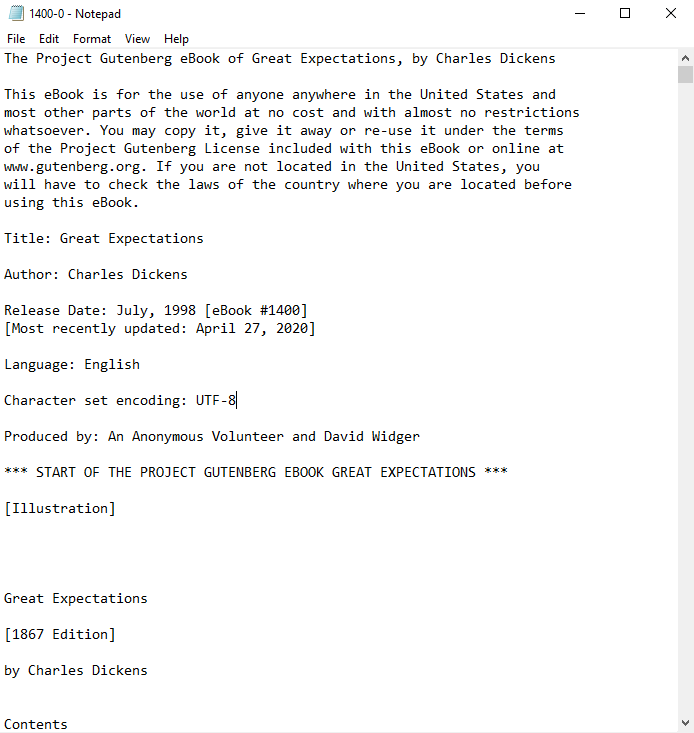
\includegraphics[width = 0.8\textwidth]{Images/data_clean_orig.PNG} % enter the filename here
		\caption{Before File Editing - Great Expectations}
		\label{fig:data-clean-orig}
	\end{center}
\end{figure}

\begin{figure}[H]
	\begin{center}
		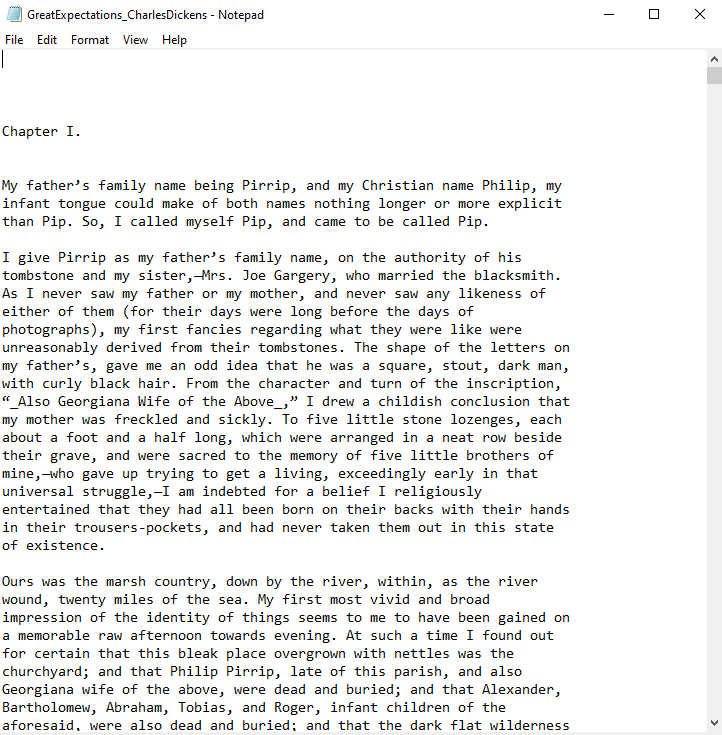
\includegraphics[width = 0.8\textwidth]{Images/data_clean_final.PNG} % enter the filename here
		\caption{After File Editing - Great Expectations}
		\label{fig:data-clean-final}
	\end{center}
\end{figure}


\subsection{Character Replacement}
\label{sec:data-clean-coding}

This is a somewhat simpler version to work with, as we perform a quick analysis of the frequency of certain outlying characters and either remove them or replace them on the basis of whether they would tentatively taint our data set, be it the training data or the testing data sets.

The way we accomplish this task is by the use of a brief Python code, which is as follows. But before we go about sharing which characters to remove or replace, let us import the right packages to accomplish this task.

\begin{code}
\label{code:libraries}
\begin{minted}[frame=single,framesep=10pt]{python}
import pandas as pd
import numpy as np
import matplotlib.pyplot as plt
import os
import math
import re
from wordcloud import WordCloud, STOPWORDS
from PIL import Image
\end{minted}
\caption{List of all libraries used in the Dissertation}
\end{code}

Next, we shall define a PATH and a list to store all the data source files in that location. This can be interchanged with the links to \textcite{project-gutenburg} as well, but that way, we would not be able to directly work with \ref{sec:data-clean-files}. From the code \ref{code:libraries}, we already have the necessary libraries imported.

\begin{code}
\label{code:data-source-location}
\begin{minted}[frame=single,framesep=10pt]{python}
PATH = '~/Dissertation/markovchain/datasets/'

all_files = os.listdir(PATH)
all_files

\end{minted}
\caption{A sample location where the data sets are being stored}
\end{code}

Finally, let us understand which characters were causing problems through the next piece of code.


\begin{code}
\label{code:data-clean}
\begin{minted}[frame=single,framesep=10pt]{python}
def data_cleaning(novel):
    
    novel = re.sub('\n', ' ', novel)
    novel = re.sub('_', ' ', novel)
    novel = re.sub('\u200a', ' ', novel)
    novel = re.sub('½', '1/2', novel)
    novel = re.sub(' +', ' ', novel)
    novel = re.sub('\t', ' ', novel)
    novel = re.sub('…', ' ', novel)
    
    return novel

\end{minted}
\caption{The characters +, \textunderscore, $\cdots$ mentioned above cause a little problem, bringing some sort of ambiguity for the same novel in the final data model. Thus, we end up replacing them}.
\end{code}


\section{List of Novels} % enter the name of the section here
\label{sec:novels-list} % enter the section label here (for cross-referencing)

Before sharing the actual word clouds, let us consider the code we shall be using for this purpose. We use the code from \ref{code:data-source-location} in order to edit out all the unnecessary characters.

\begin{code}
\label{code:word-cloud}
\begin{minted}[frame=single,framesep=10pt]{python}
for file in all_files:
            
    book = open(PATH + file, 'r', encoding = 'utf-8-sig')
    novel = book.read()
    
    novel = re.sub('\n', ' ', novel)
    novel = re.sub('_', ' ', novel)
    novel = re.sub('\u200a', ' ', novel)
    novel = re.sub('½', '1/2', novel)
    novel = re.sub(' +', ' ', novel)
    novel = re.sub('\t', ' ', novel)
    novel = re.sub('…', ' ', novel)
    
    word_cloud = WordCloud(
        width=3000,
        height=2000,
        random_state=123,
        max_words=100,
        background_color="purple",
        colormap="Set2",
        collocations=False,
        stopwords=STOPWORDS
    ).generate(novel)
    
    word_cloud.to_file(f'{file[:-4]}.jpeg')
    
\end{minted}
\caption{The characters +, \textunderscore, $\cdots$ mentioned above cause a little problem, bringing some sort of ambiguity for the same novel in the final data model. Thus, we end up replacing them}.
\end{code}

\begin{code}
\label{code:histograms}
\begin{minted}[frame=single,framesep=10pt]{python}
for file in all_files:
    
    dflux = charslen_df[file]
    dflux2 = charslen_df[file].loc[charslen_df[file] < 10000]
    dflux3 = charslen_df[file].loc[charslen_df[file] < 1000]
    dflux4 = charslen_df[file].loc[charslen_df[file] < 100]


    fig, axes = plt.subplots(1, 4)
    plt.rcParams["figure.figsize"] = (20,4)
    plt.title(f'{file[:-4]}')

    dflux.hist(bins=10, ax=axes[0])
    dflux2.hist(bins=10, ax=axes[1])
    dflux3.hist(bins=10, ax=axes[2])
    dflux4.hist(bins=10, ax=axes[3])
    
    plt.savefig(f'char_hist_{file[:-4]}.jpeg', bbox_inches='tight')
    
\end{minted}
\caption{All of our histograms are being divided into 4 slicings for a better understanding of the character frequencies}.
\end{code}

We are using 8 novels in our Natural Language Processing model, which heavily relies on character analysis. A list of the books we use is as follows:

\begin{itemize}
    \item \textcite{great_expectations}
    \item \textcite{great-gatsby}
    \item \textcite{huckleberry-finn}
    \item \textcite{moby-dick}
    \item \textcite{pride-prejudice}
    \item \textcite{sherlock-holmes}
    \item \textcite{sign-of-the-four}
    \item \textcite{oliver-twist}
\end{itemize}

We created some word clouds for each book, and we shall briefly go over a short summary of each novel. One key thing to note is all these novels are available for reading widely. Their publishing rights have lapsed since the year mentioned next to each novel and are available in the public domain for anyone to read.

Additionally, we have also created some character occurrence frequencies, varying from the complete dataset to certain sections of them. They would be available in the images following the word clouds. Let us also look at just one example of a Histogram for character frequencies in this novel. Here, we are working with character frequencies in 4 stages.

\begin{itemize}
    \item \textbf{Complete Frequency}
    \item \textbf{Frequency $<$ 10000 in occurrence}
    \item \textbf{Frequency $<$ 1000 in occurrence}
    \item \textbf{Frequency $<$ 100 in occurrence}
\end{itemize}
 
\subsection{\textcite{great_expectations}} %enter the name of the subsection here
\label{sec:great-expectations} % enter the subsection label here (for cross-referencing)

Great Expectations follows the childhood and young adult years of Pip a blacksmith's apprentice in a country village. He suddenly comes into a large fortune (his great expectations) from a mysterious benefactor and moves to London where he enters high society. He thinks he knows where the money has come from but he turns out to be sadly mistaken. The story also follows Pip's dealings with Estella, a young woman he adores but who cannot return his love. \textcite{great_expectations-summary}. Below is a quick word cloud from the complete book. 

\begin{figure}[H]
	\begin{center}
		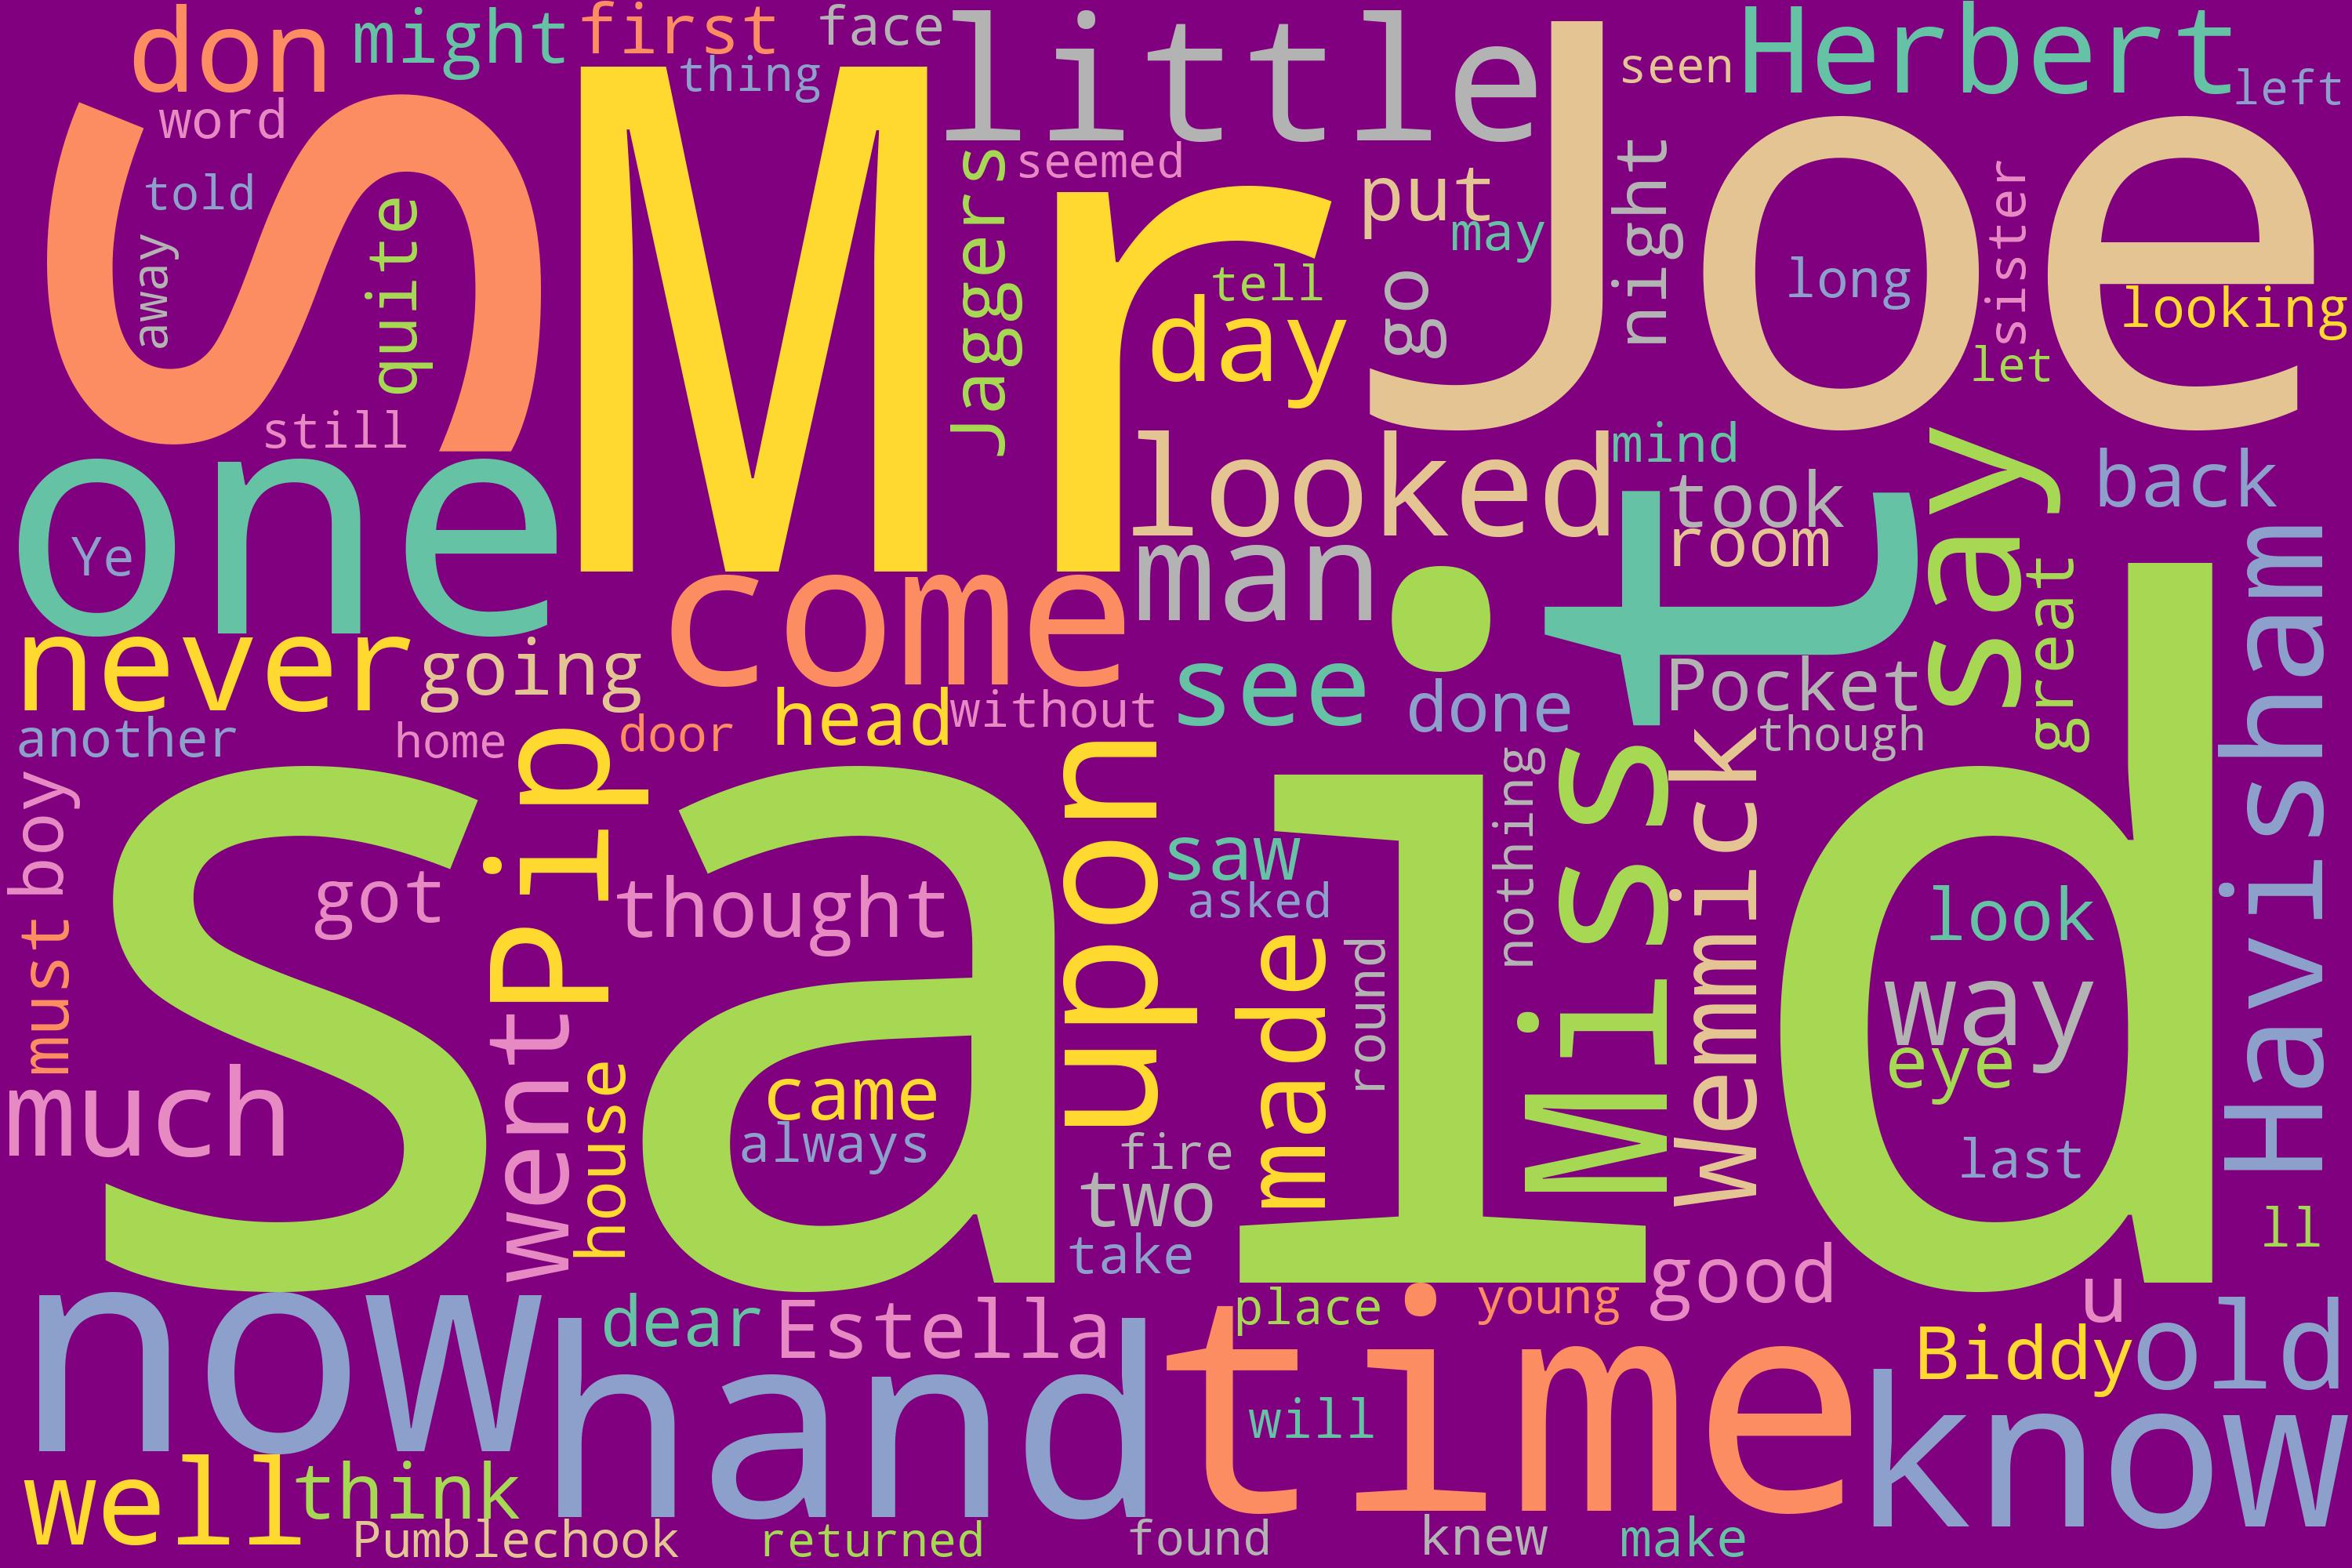
\includegraphics[width = 0.7\textwidth]{Images/GreatExpectations_CharlesDickens.jpeg} % enter the filename here
		\caption{Word Cloud - Great Expectations}
		\label{fig:great-expectations}
	\end{center}
\end{figure}

In Great Expectations, we do see Pip, who is a very prominent character in the book, along with his counterpart, Estella.

\begin{figure}[H]
	\begin{center}
		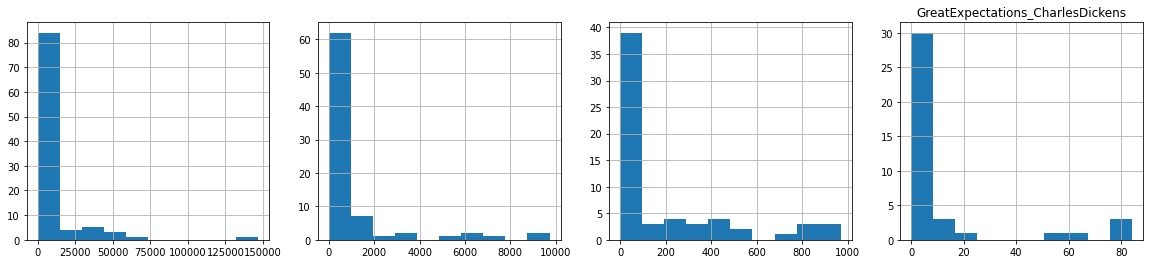
\includegraphics[width = 1.0\textwidth]{Images/char_hist_GreatExpectations_CharlesDickens.jpeg} % enter the filename here
		\caption{Character Histogram - Great Expectations}
		\label{fig:histogram-greatexp}
	\end{center}
\end{figure}

\subsection{\textcite{great-gatsby}} %enter the name of the subsection here
\label{sec:great-gatsby} % enter the subsection label here (for cross-referencing)

F. Scott Fitzgerald's novel, The Great Gatsby, follows Jay Gatsby, a man who orders his life around one desire: to be reunited with Daisy Buchanan, the love he lost five years earlier. Gatsby's quest leads him from poverty to wealth, into the arms of his beloved, and eventually to death. Published in 1925, The Great Gatsby is a classic piece of American fiction. It is a novel of triumph and tragedy, noted for the remarkable way Fitzgerald captured a cross-section of American society. \textcite{great-gatsby-summary}. Below is a quick word cloud from the complete book. 

\begin{figure}[H]
	\begin{center}
		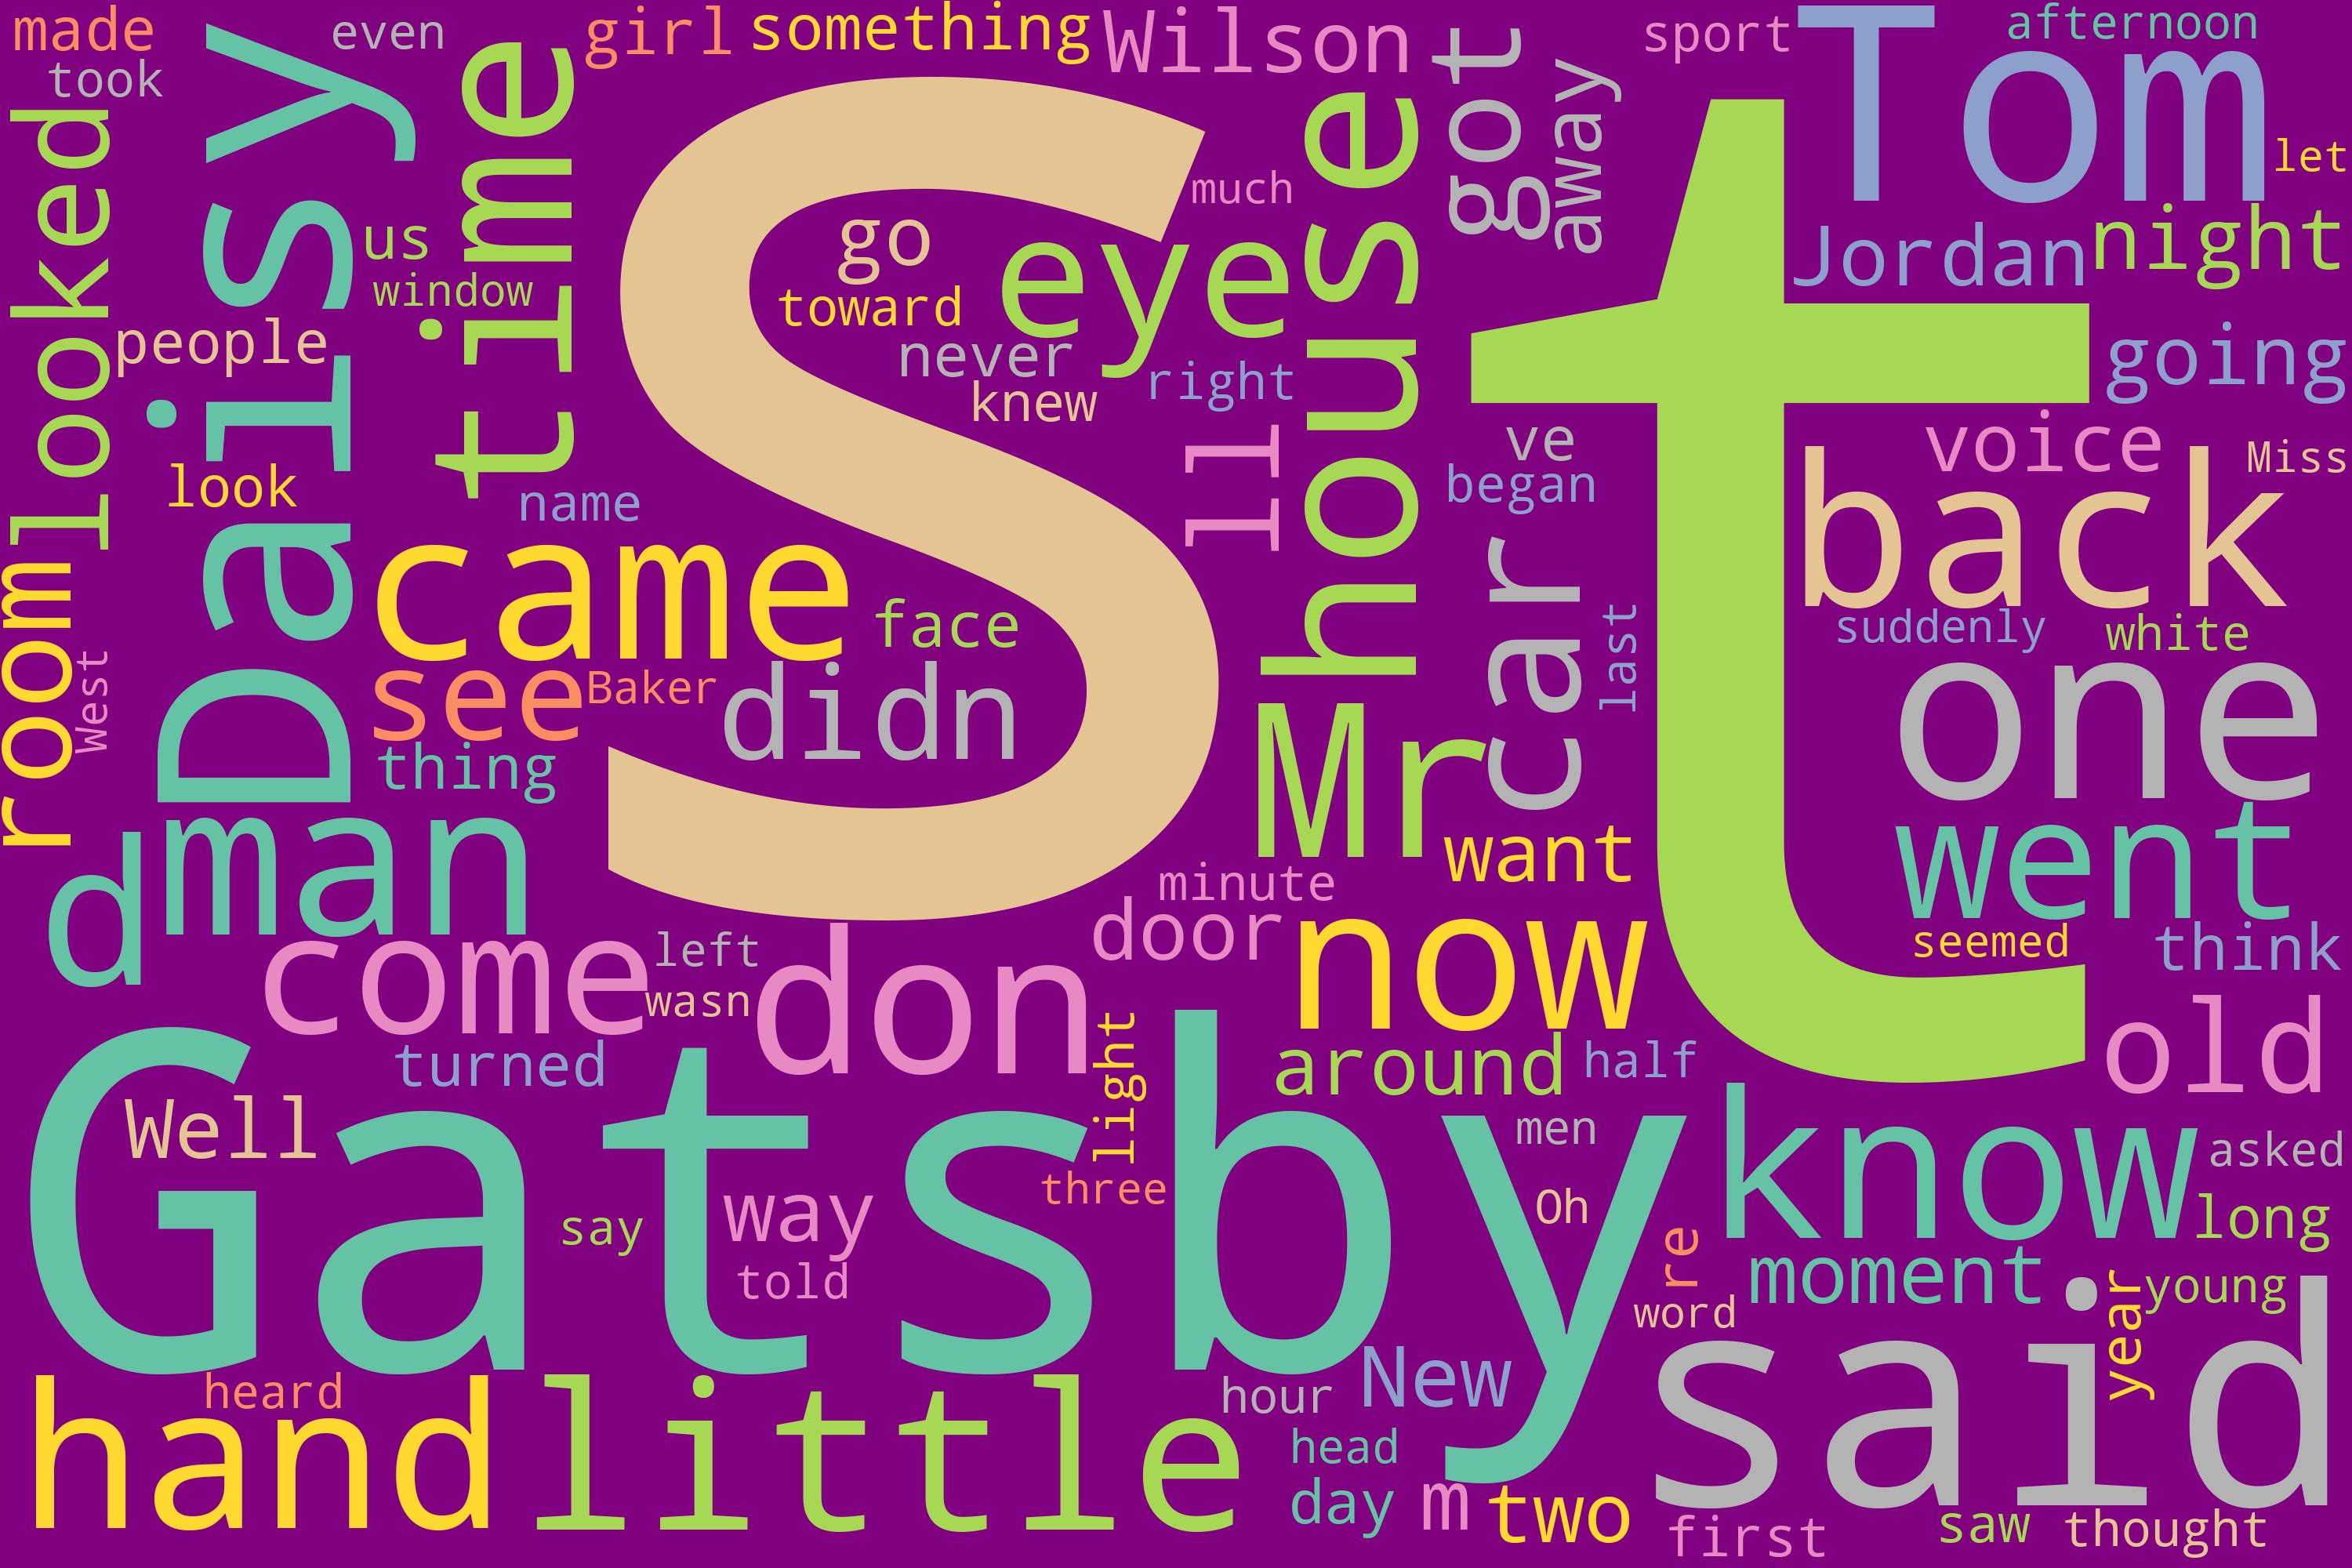
\includegraphics[width = 0.7\textwidth]{Images/GreatGatsby_FScottFitzgerald.jpeg} % enter the filename here
		\caption{Word Cloud - Great Gatsby}
		\label{fig:great-gatsby}
	\end{center}
\end{figure}

\begin{figure}[H]
	\begin{center}
		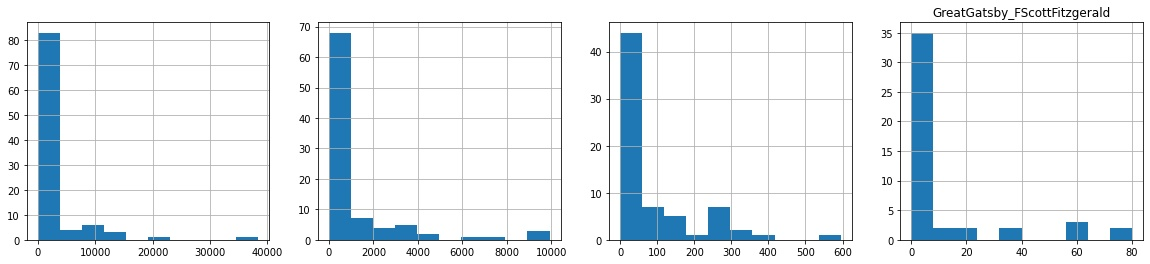
\includegraphics[width = 1.0\textwidth]{Images/char_hist_GreatGatsby_FScottFitzgerald.jpeg} % enter the filename here
		\caption{Character Histogram - Great Gatsby}
		\label{fig:histogram-greatgatsby}
	\end{center}
\end{figure}


\subsection{\textcite{huckleberry-finn}} %enter the name of the subsection here
\label{sec:huckleberry-finn} % enter the subsection label here (for cross referencing)

The book’s narrator is Huckleberry Finn, a youngster whose artless vernacular speech is admirably adapted to detailed and poetic descriptions of scenes, vivid representations of characters, and narrative renditions that are both broadly comic and subtly ironic. The book’s pages are dotted with idyllic descriptions of a great river and the surrounding forests, Huck’s good nature, and unconscious humor. But a thread that runs through adventure after the adventure is that of human cruelty, which shows itself both in the acts of individuals and in their unthinking acceptance of such institutions as slavery. \textcite{huckleberry-finn-summary}. Below is a quick word cloud from the complete book. 

\begin{figure}[H]
	\begin{center}
		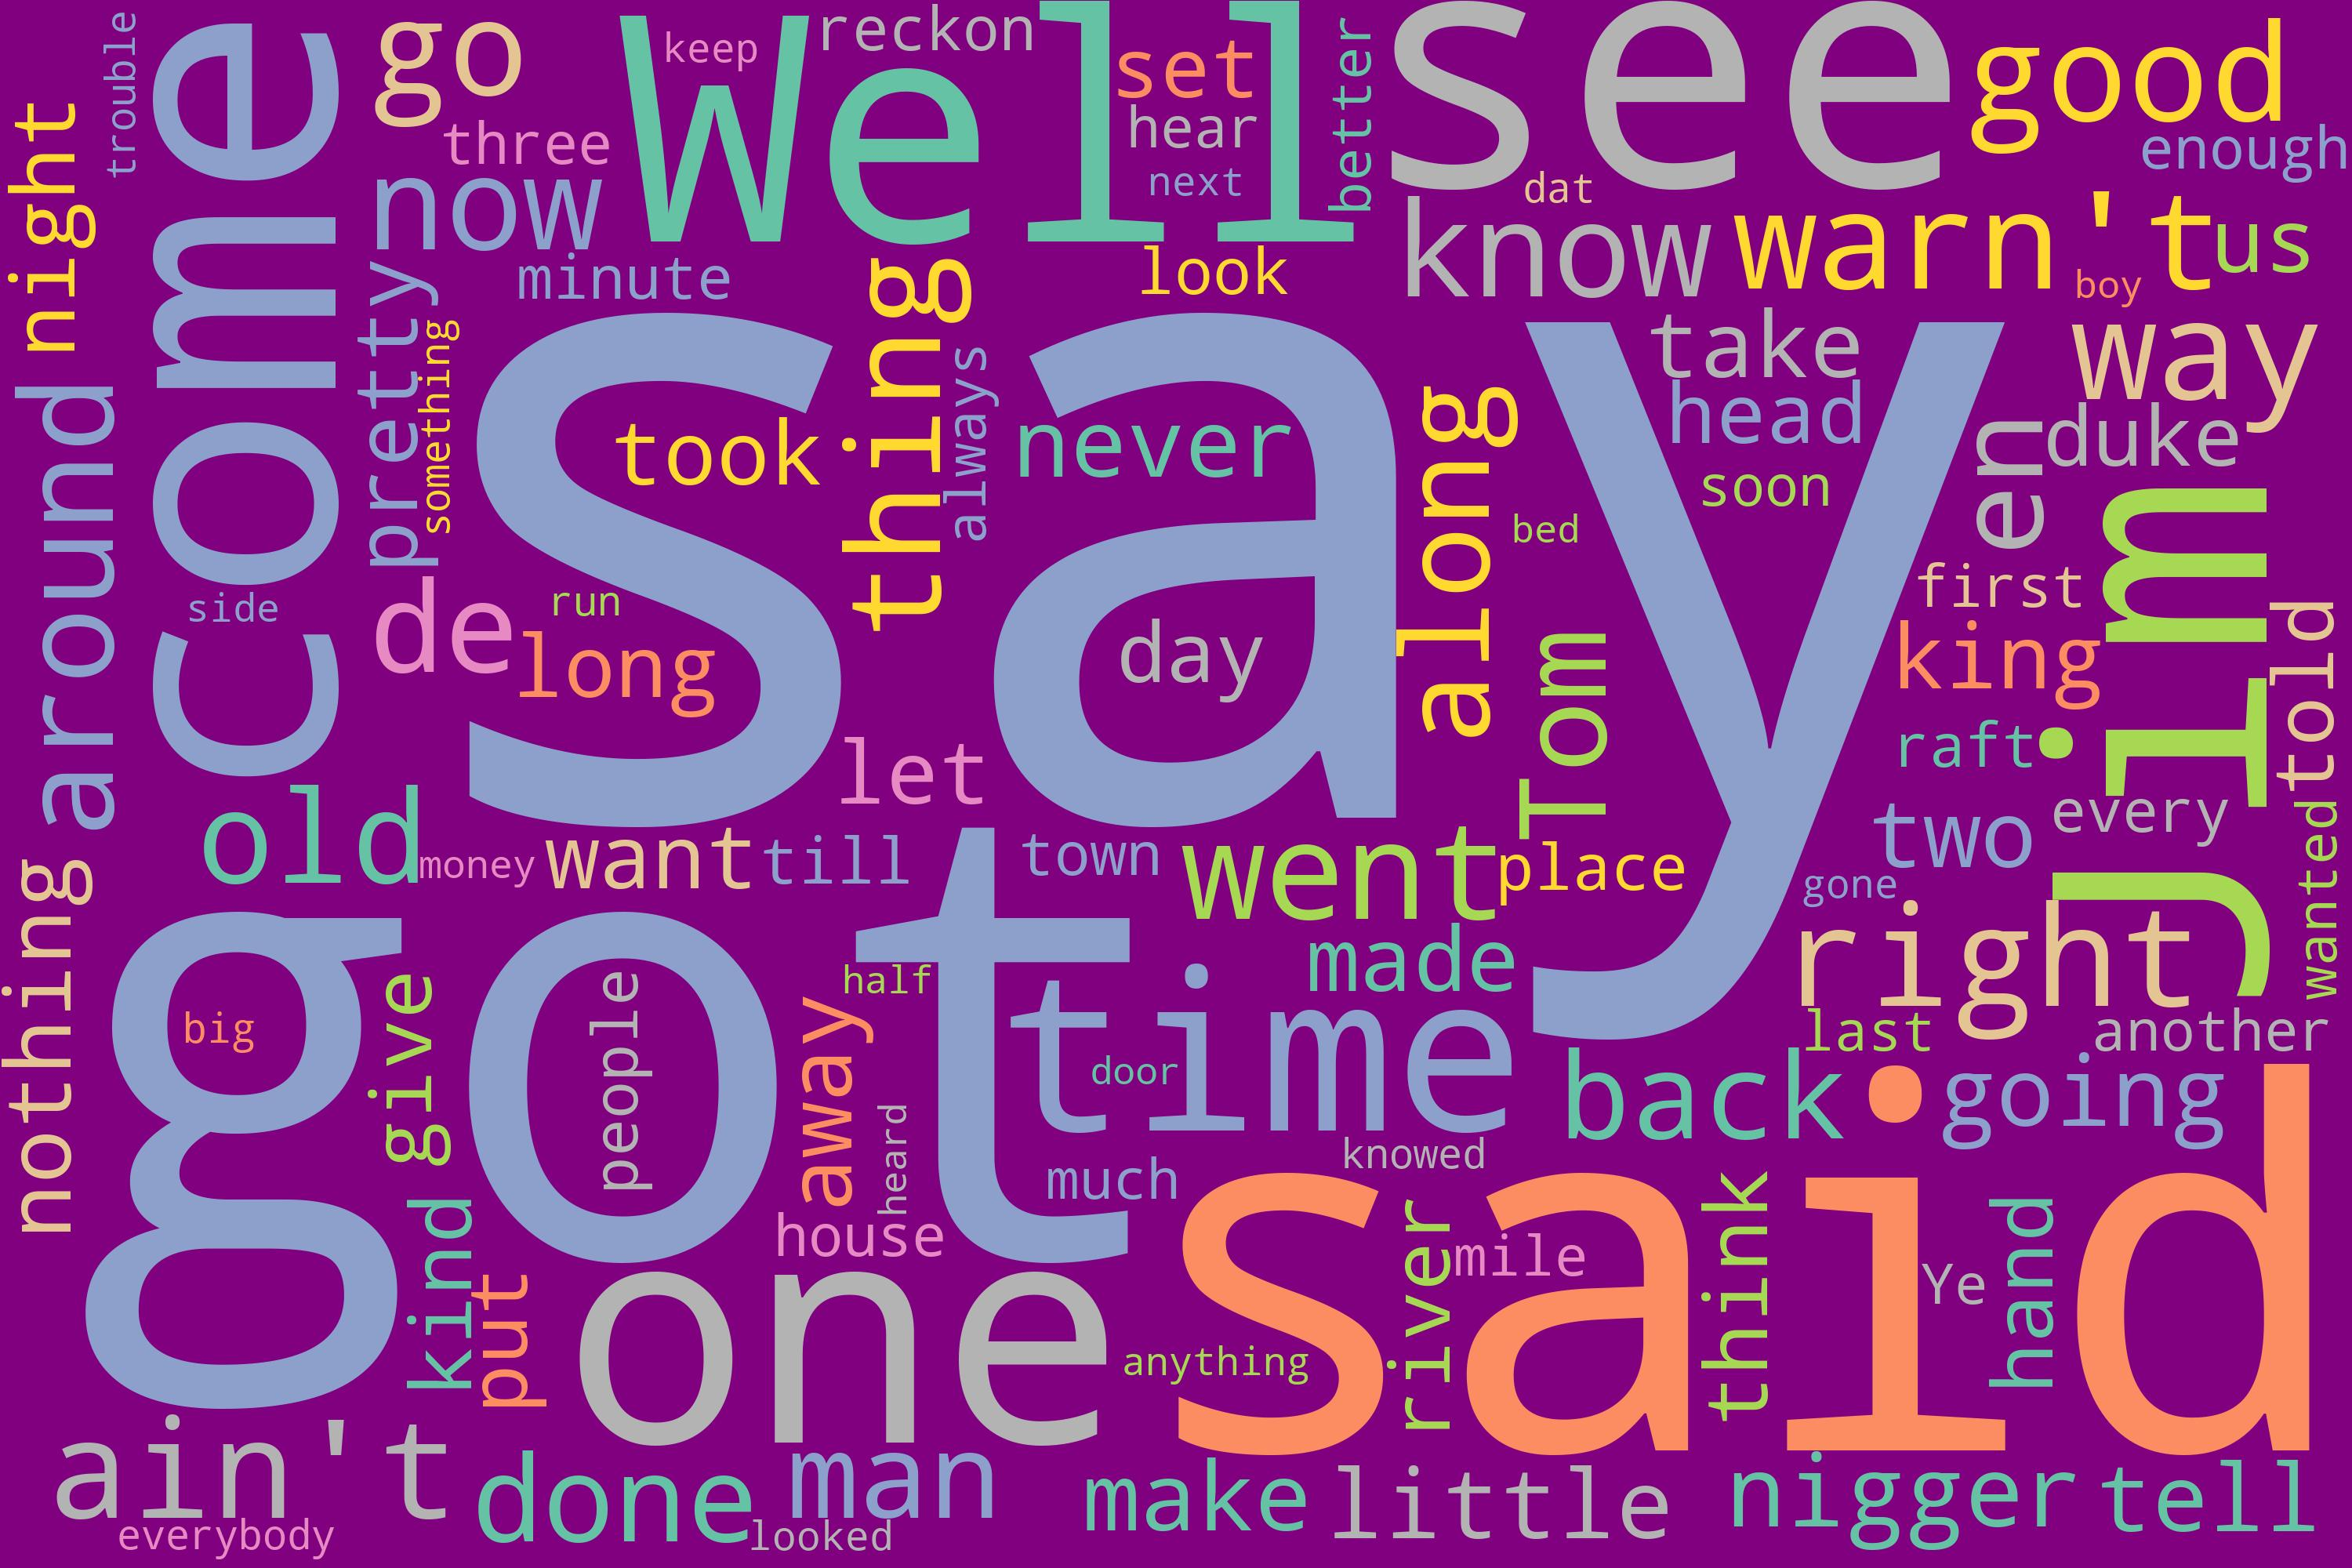
\includegraphics[width = 0.7\textwidth]{Images/HuckleberryFinn_MarkTwain.jpeg} % enter the filename here
		\caption{Word Cloud - Huckleberry Finn}
		\label{fig:huckleberry-finn}
	\end{center}
\end{figure}

\begin{figure}[H]
	\begin{center}
		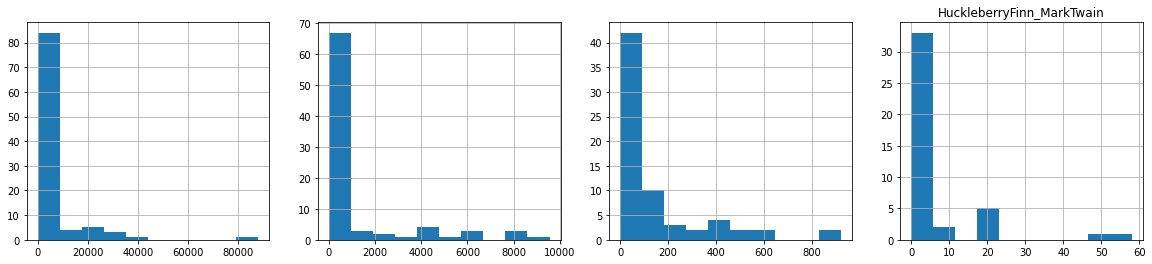
\includegraphics[width = 1.0\textwidth]{Images/char_hist_HuckleberryFinn_MarkTwain.jpeg} % enter the filename here
		\caption{Character Histogram - Huckleberry Finn}
		\label{fig:histogram-huckbfinn}
	\end{center}
\end{figure}

\subsection{\textcite{moby-dick}} %enter the name of the subsection here
\label{sec:moby-dick} % enter the subsection label here (for cross referencing)

Moby Dick famously begins with the narratorial invocation “Call me Ishmael.” The narrator, like his biblical counterpart, is an outcast. Ishmael, who turns to the sea for meaning, relays to the audience the final voyage of the Pequod, a whaling vessel. Amid a story of tribulation, beauty, and madness, the reader is introduced to a number of characters, many of whom have names with religious resonance. Moby Dick can sustain numerous, if not seemingly infinite, readings generated by multiple interpretative approaches. One of the most fruitful ways to appreciate the novel’s complexity is through the names that Melville gave to its characters, many of which are shared with figures of the Abrahamic religions. \textcite{moby-dick-summary}. Below is a quick word cloud from the complete book. 

\begin{figure}[H]
	\begin{center}
		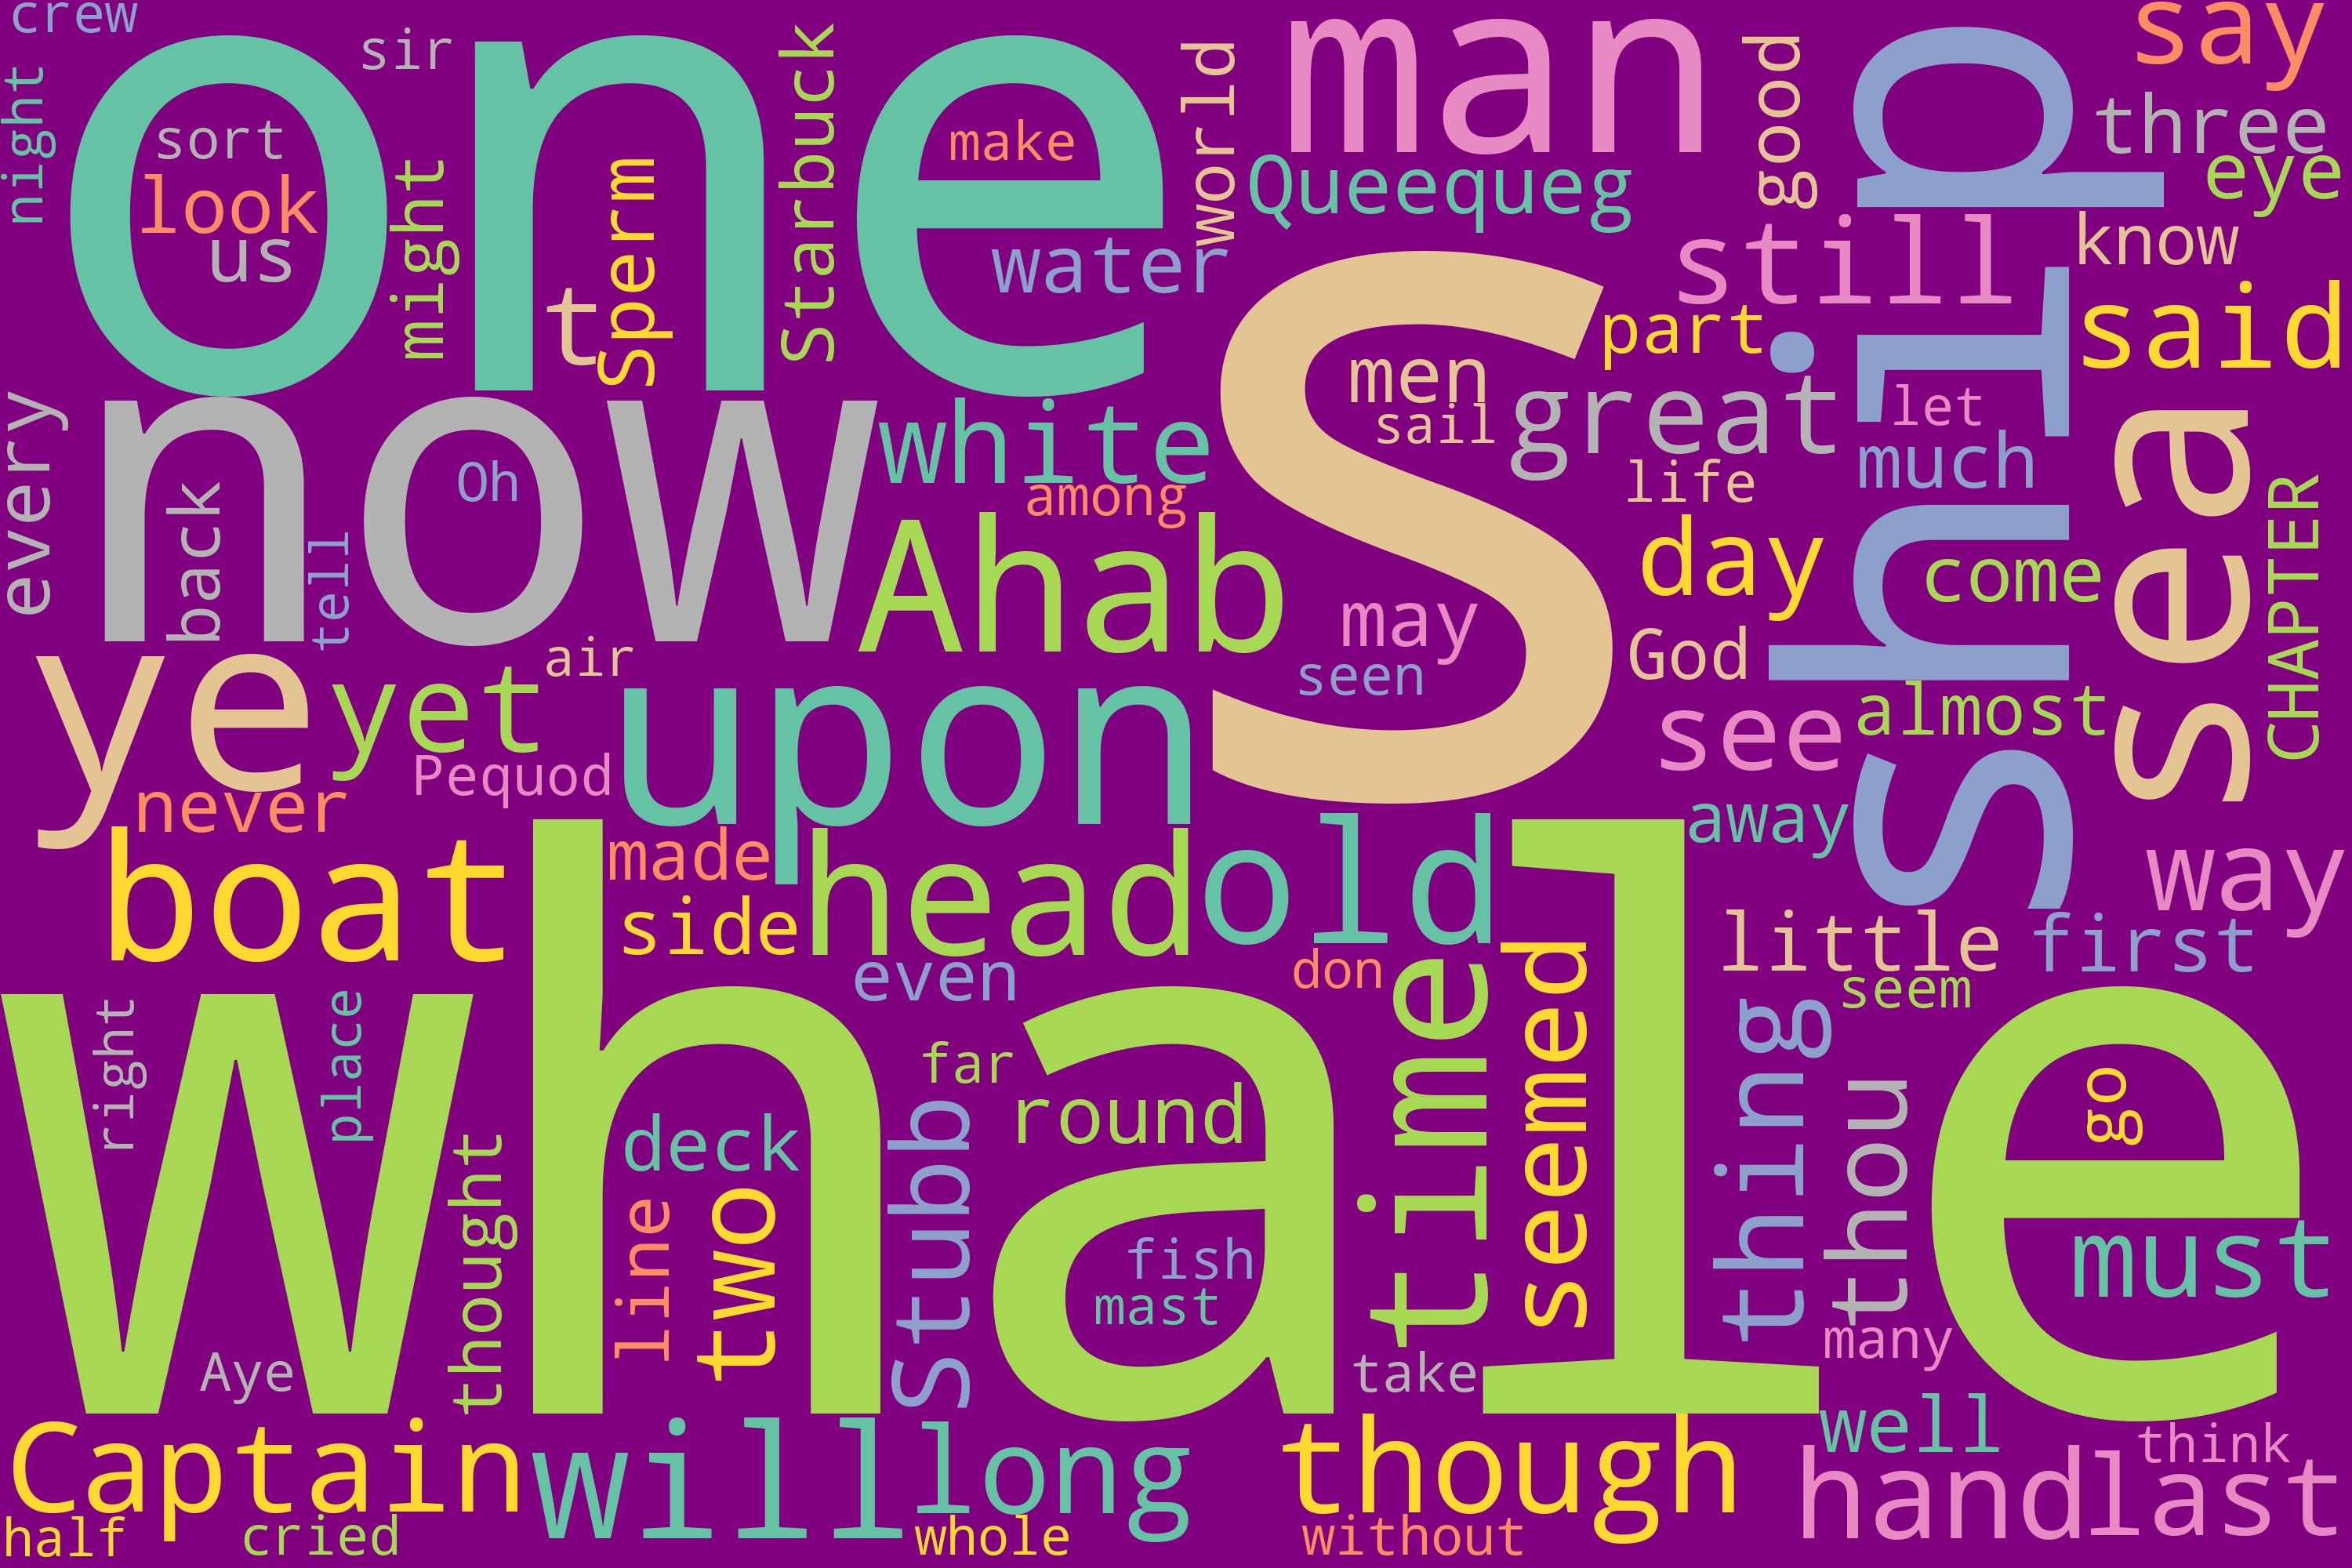
\includegraphics[width = 0.7\textwidth]{Images/MobyDick_HermanMelville.jpeg} % enter the filename here
		\caption{Word Cloud - Moby Dick}
		\label{fig:moby-dick}
	\end{center}
\end{figure}

\begin{figure}[H]
	\begin{center}
		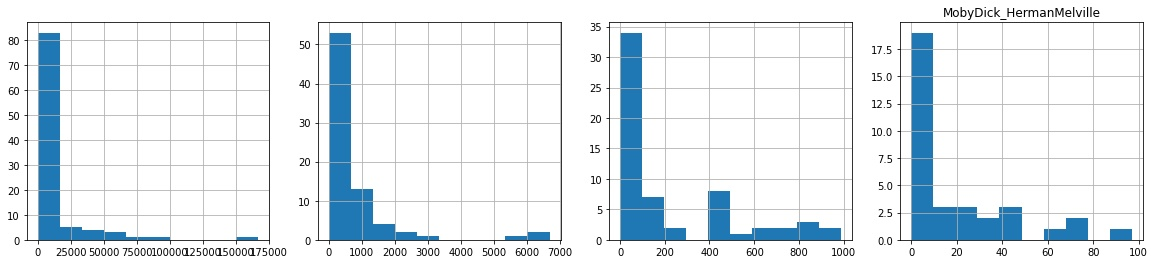
\includegraphics[width = 1.0\textwidth]{Images/char_hist_MobyDick_HermanMelville.jpeg} % enter the filename here
		\caption{Character Histogram - Moby Dick}
		\label{fig:histogram-mobydick}
	\end{center}
\end{figure}


\subsection{\textcite{oliver-twist}} %enter the name of the subsection here
\label{sec:oliver-twist} % enter the subsection label here (for cross referencing)

The novel follows the journey of the titular character, Oliver Twist. Oliver, an orphan since birth, spends much of his childhood at a “child farm” (orphanage) with too many children and too little food. The farm is located roughly 70 miles outside London. Charles Dickens was well versed in the poverty of London, as he himself was a child worker after his father was sent to debtors’ prison. His appreciation of the hardships endured by impoverished citizens stayed with him for the rest of his life and was evident in his journalistic writings and novels. \textcite{oliver-twist-summary}. Below is a quick word cloud from the complete book. 

\begin{figure}[H]
	\begin{center}
		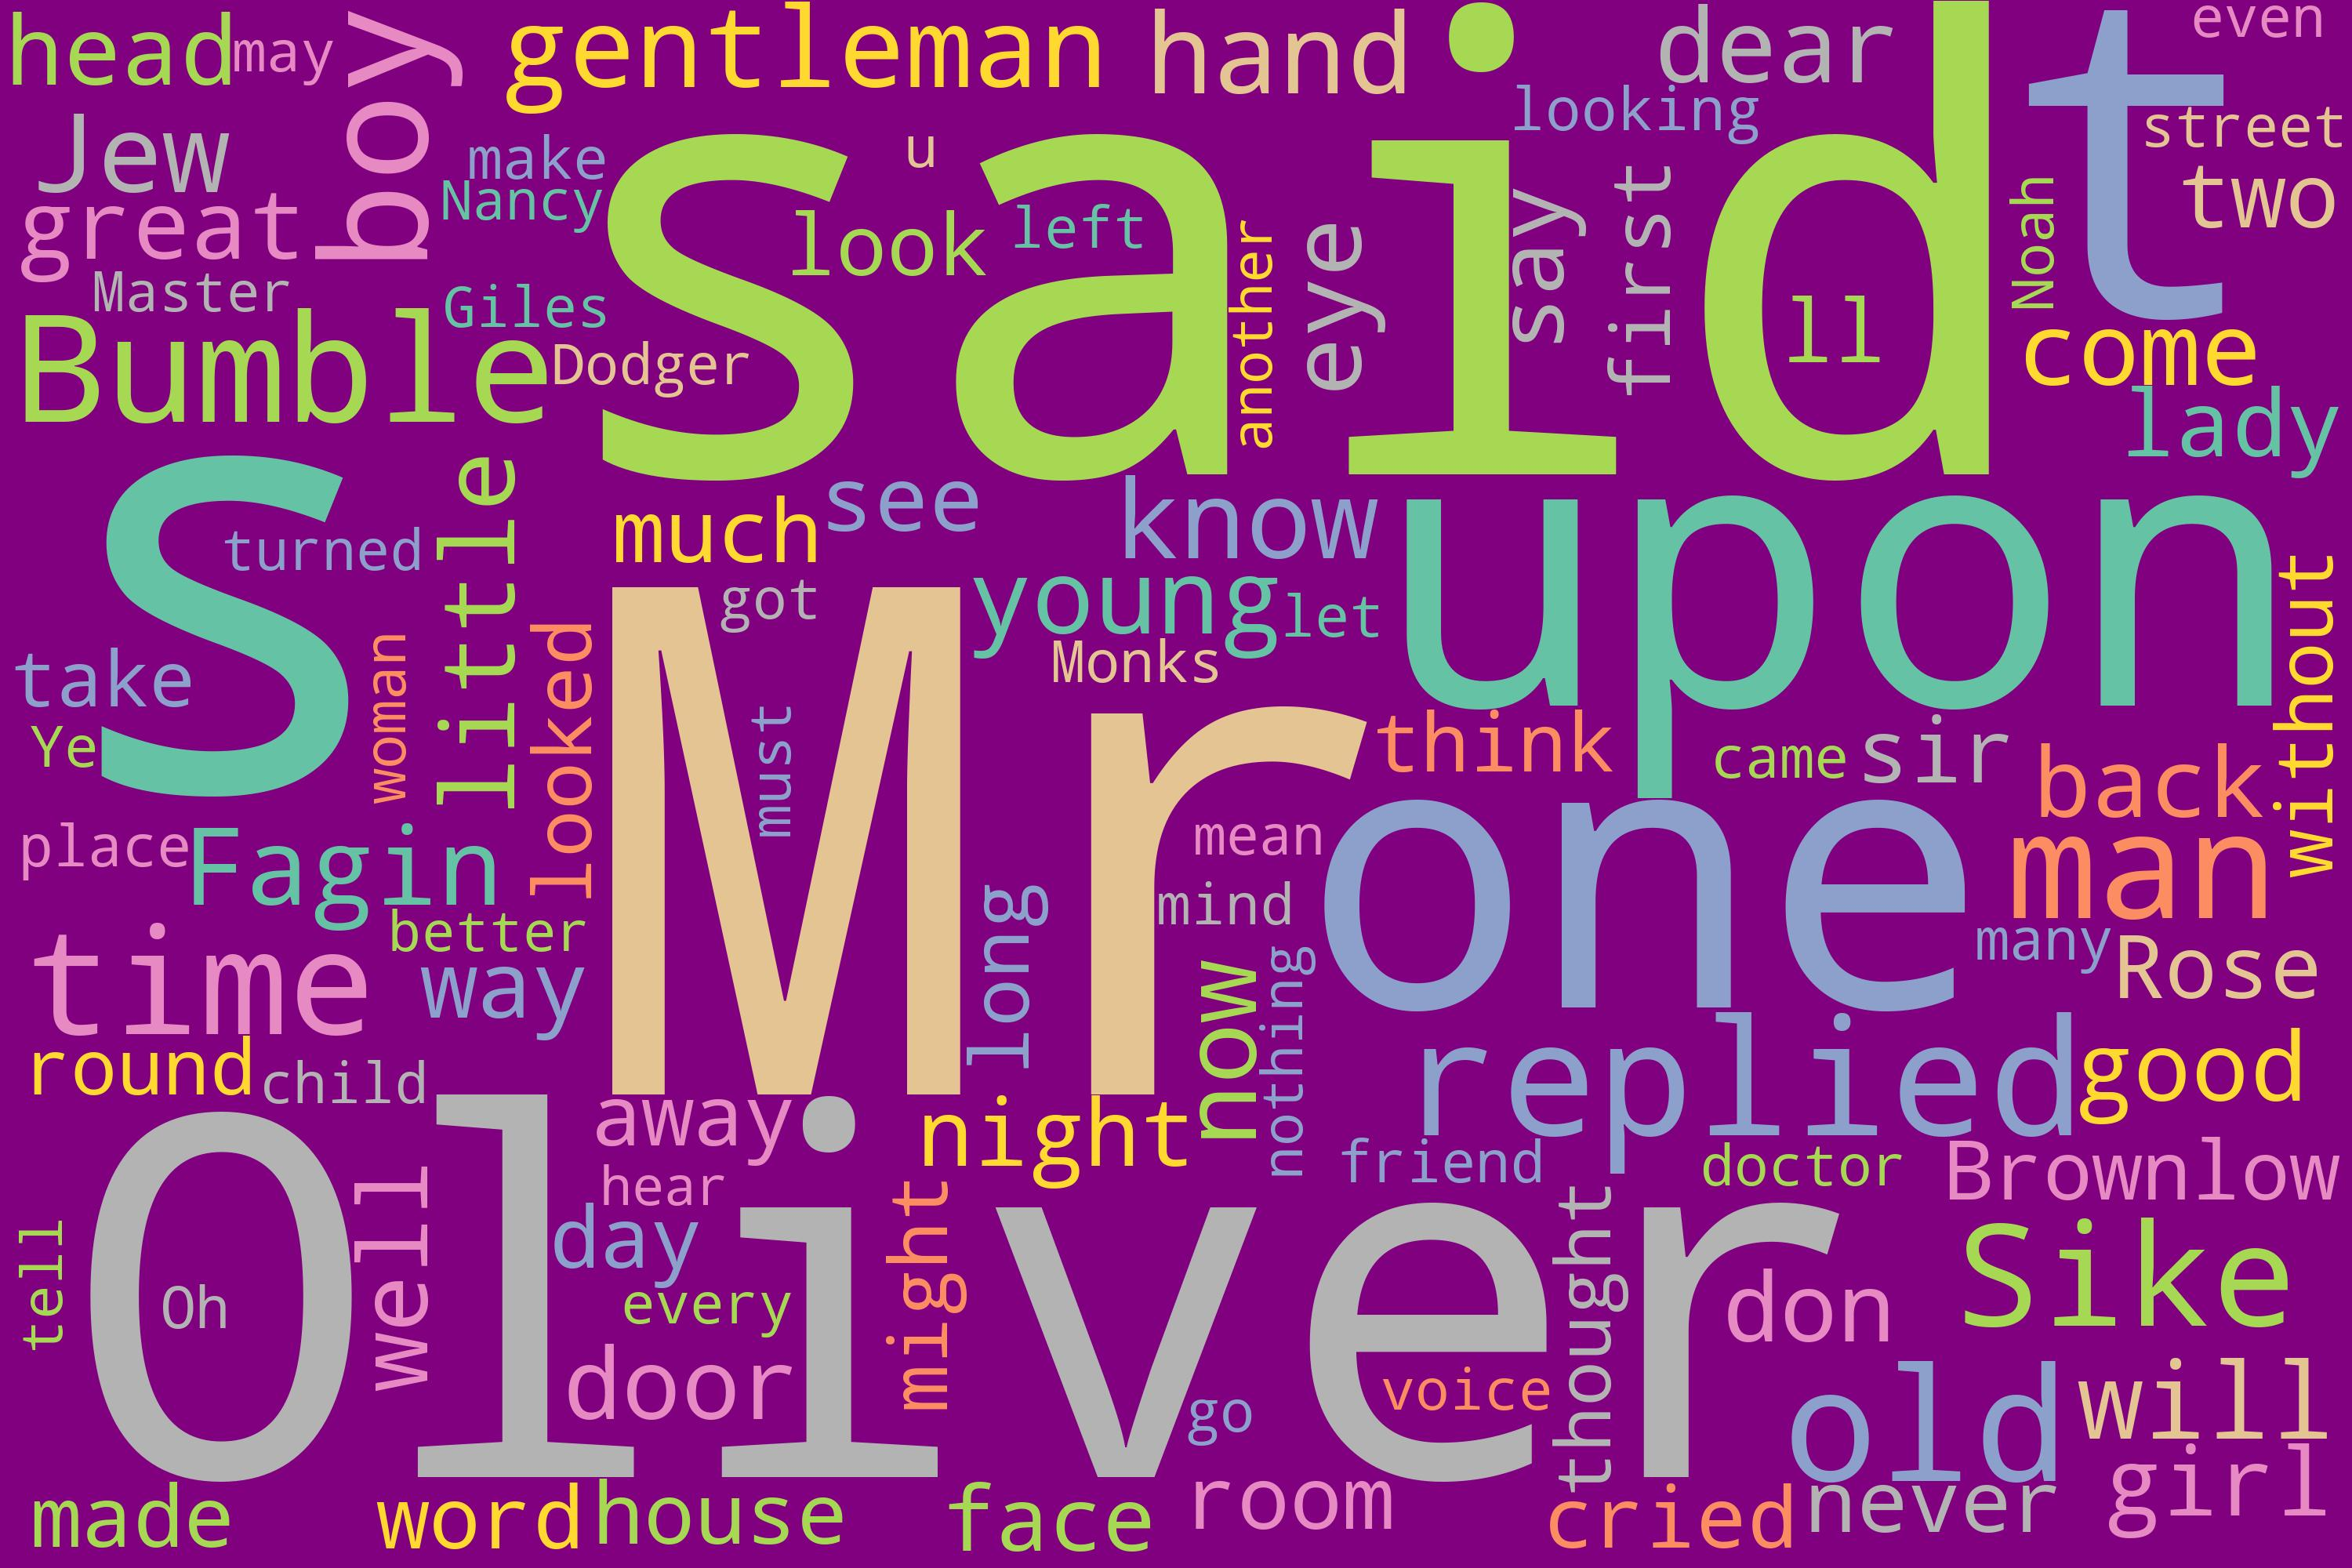
\includegraphics[width = 0.7\textwidth]{Images/OliverTwist_CharlesDickens.jpeg} % enter the filename here
		\caption{Word Cloud - Oliver Twist}
		\label{fig:oliver-twist}
	\end{center}
\end{figure}

\begin{figure}[H]
	\begin{center}
		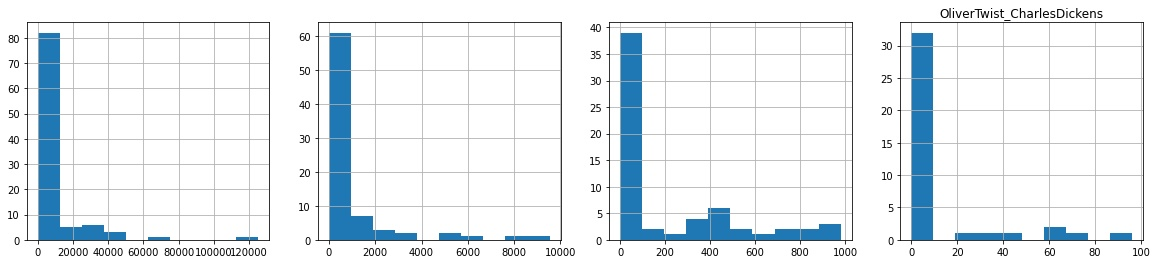
\includegraphics[width = 1.0\textwidth]{Images/char_hist_OliverTwist_CharlesDickens.jpeg} % enter the filename here
		\caption{Character Histogram - Oliver Twist}
		\label{fig:histogram-olivertwist}
	\end{center}
\end{figure}


\subsection{\textcite{pride-prejudice}} %enter the name of the subsection here
\label{sec:pride-prejudice} % enter the subsection label here (for cross referencing)

Pride and Prejudice is set in rural England at the turn of the 19th century, and it follows the Bennet family, which includes five very different sisters. The novel opens with one of the most famous lines in English literature: “It is a truth universally acknowledged, that a single man in possession of a good fortune, must be in want of a wife.” The work, which Austen initially titled First Impressions, is the second of four novels that Austen published during her lifetime. \textcite{pride-prejudice-summary}. Below is a quick word cloud from the complete book. 

\begin{figure}[H]
	\begin{center}
		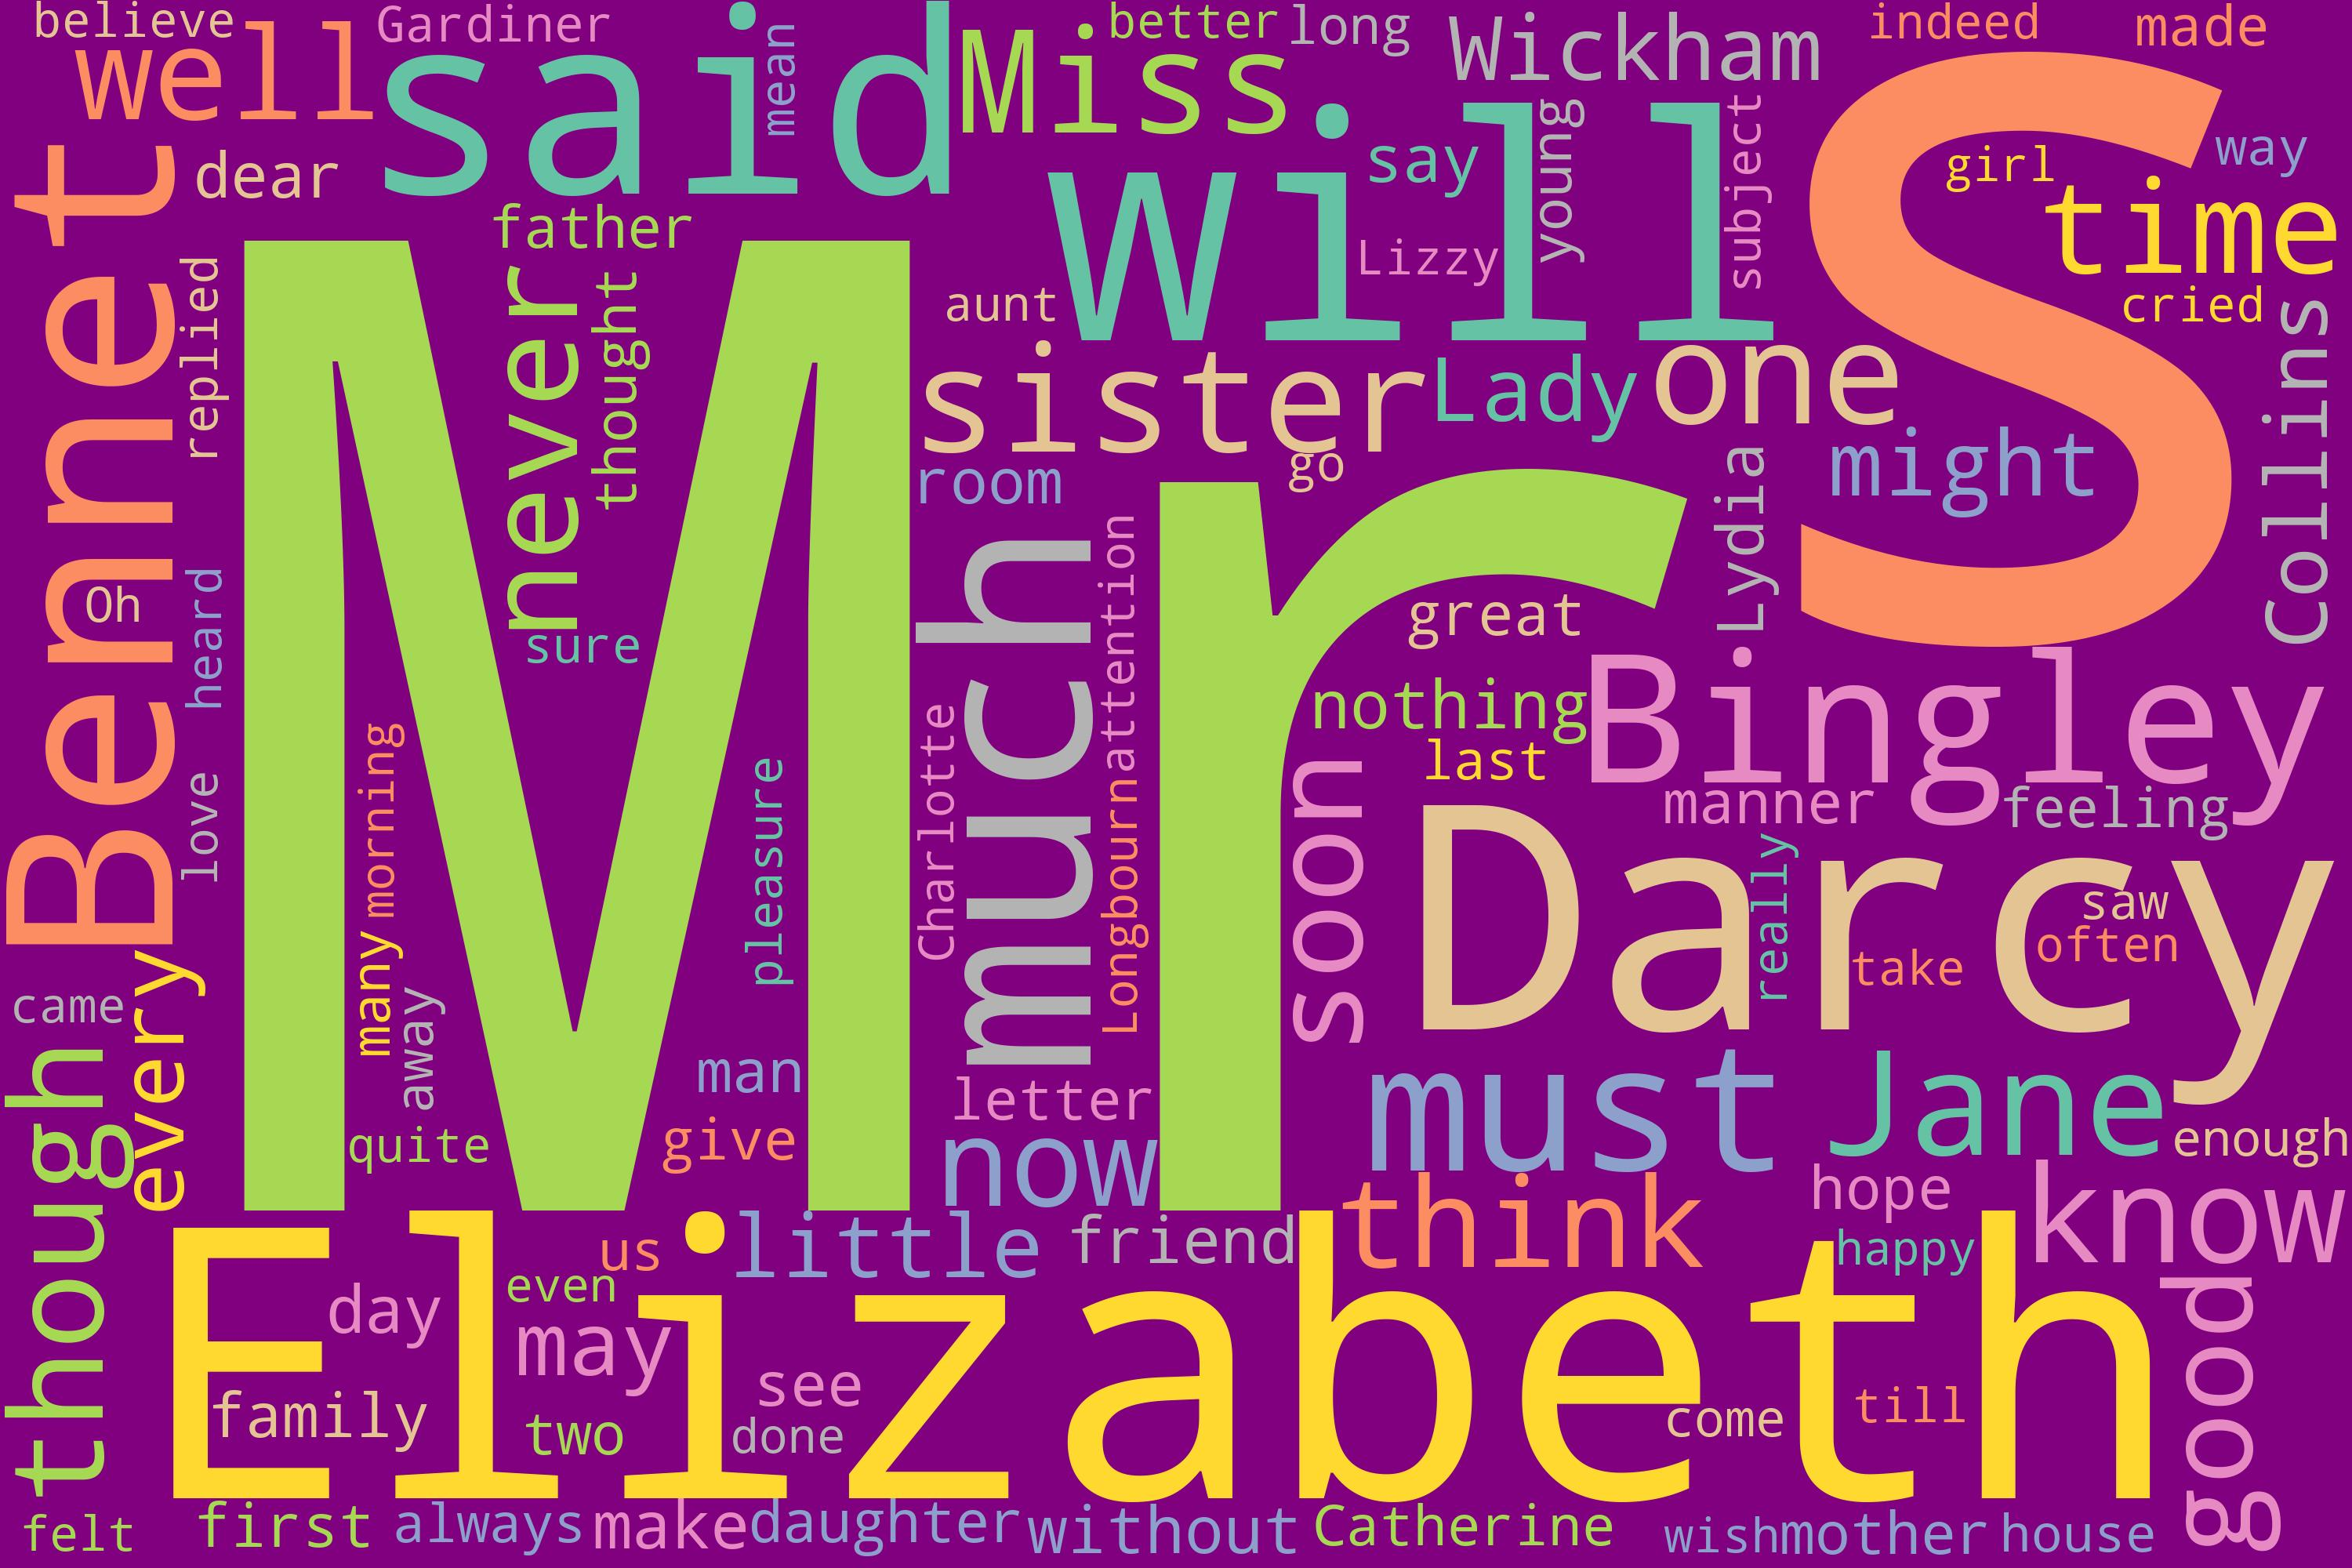
\includegraphics[width = 0.7\textwidth]{Images/PridePrejudice_JaneAusten.jpeg} % enter the filename here
		\caption{Word Cloud - Pride and Prejudice}
		\label{fig:pride-prejudice}
	\end{center}
\end{figure}

\begin{figure}[H]
	\begin{center}
		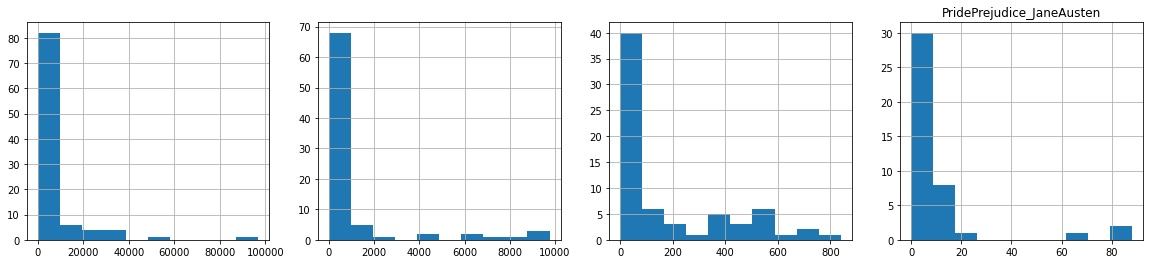
\includegraphics[width = 1.0\textwidth]{Images/char_hist_PridePrejudice_JaneAusten.jpeg} % enter the filename here
		\caption{Character Histogram - Pride and Prejudice}
		\label{fig:histogram-prideprejudice}
	\end{center}
\end{figure}



\subsection{\textcite{sherlock-holmes}} %enter the name of the subsection here
\label{sec:sherlock-holmes} % enter the subsection label here (for cross referencing)

The Adventures of Sherlock Holmes is a collection of twelve stories involving the famous London detective Sherlock Holmes and his associate Dr. Watson. The collection was published in October 1892, although the first Sherlock story appeared in the Strand Magazine in July 1891. In fact, the character of Sherlock Holmes first appeared in a short story called, A Study in Scarlet, published in Beeton's Christmas Annual in 1887. The themes of Sherlock Holmes are centered around four aspects, namely, Social Class, Justice, Deception, and Logic & Reason. \textcite{sherlock-holmes-summary}. Below is a quick word cloud from the complete book. 

\begin{figure}[H]
	\begin{center}
		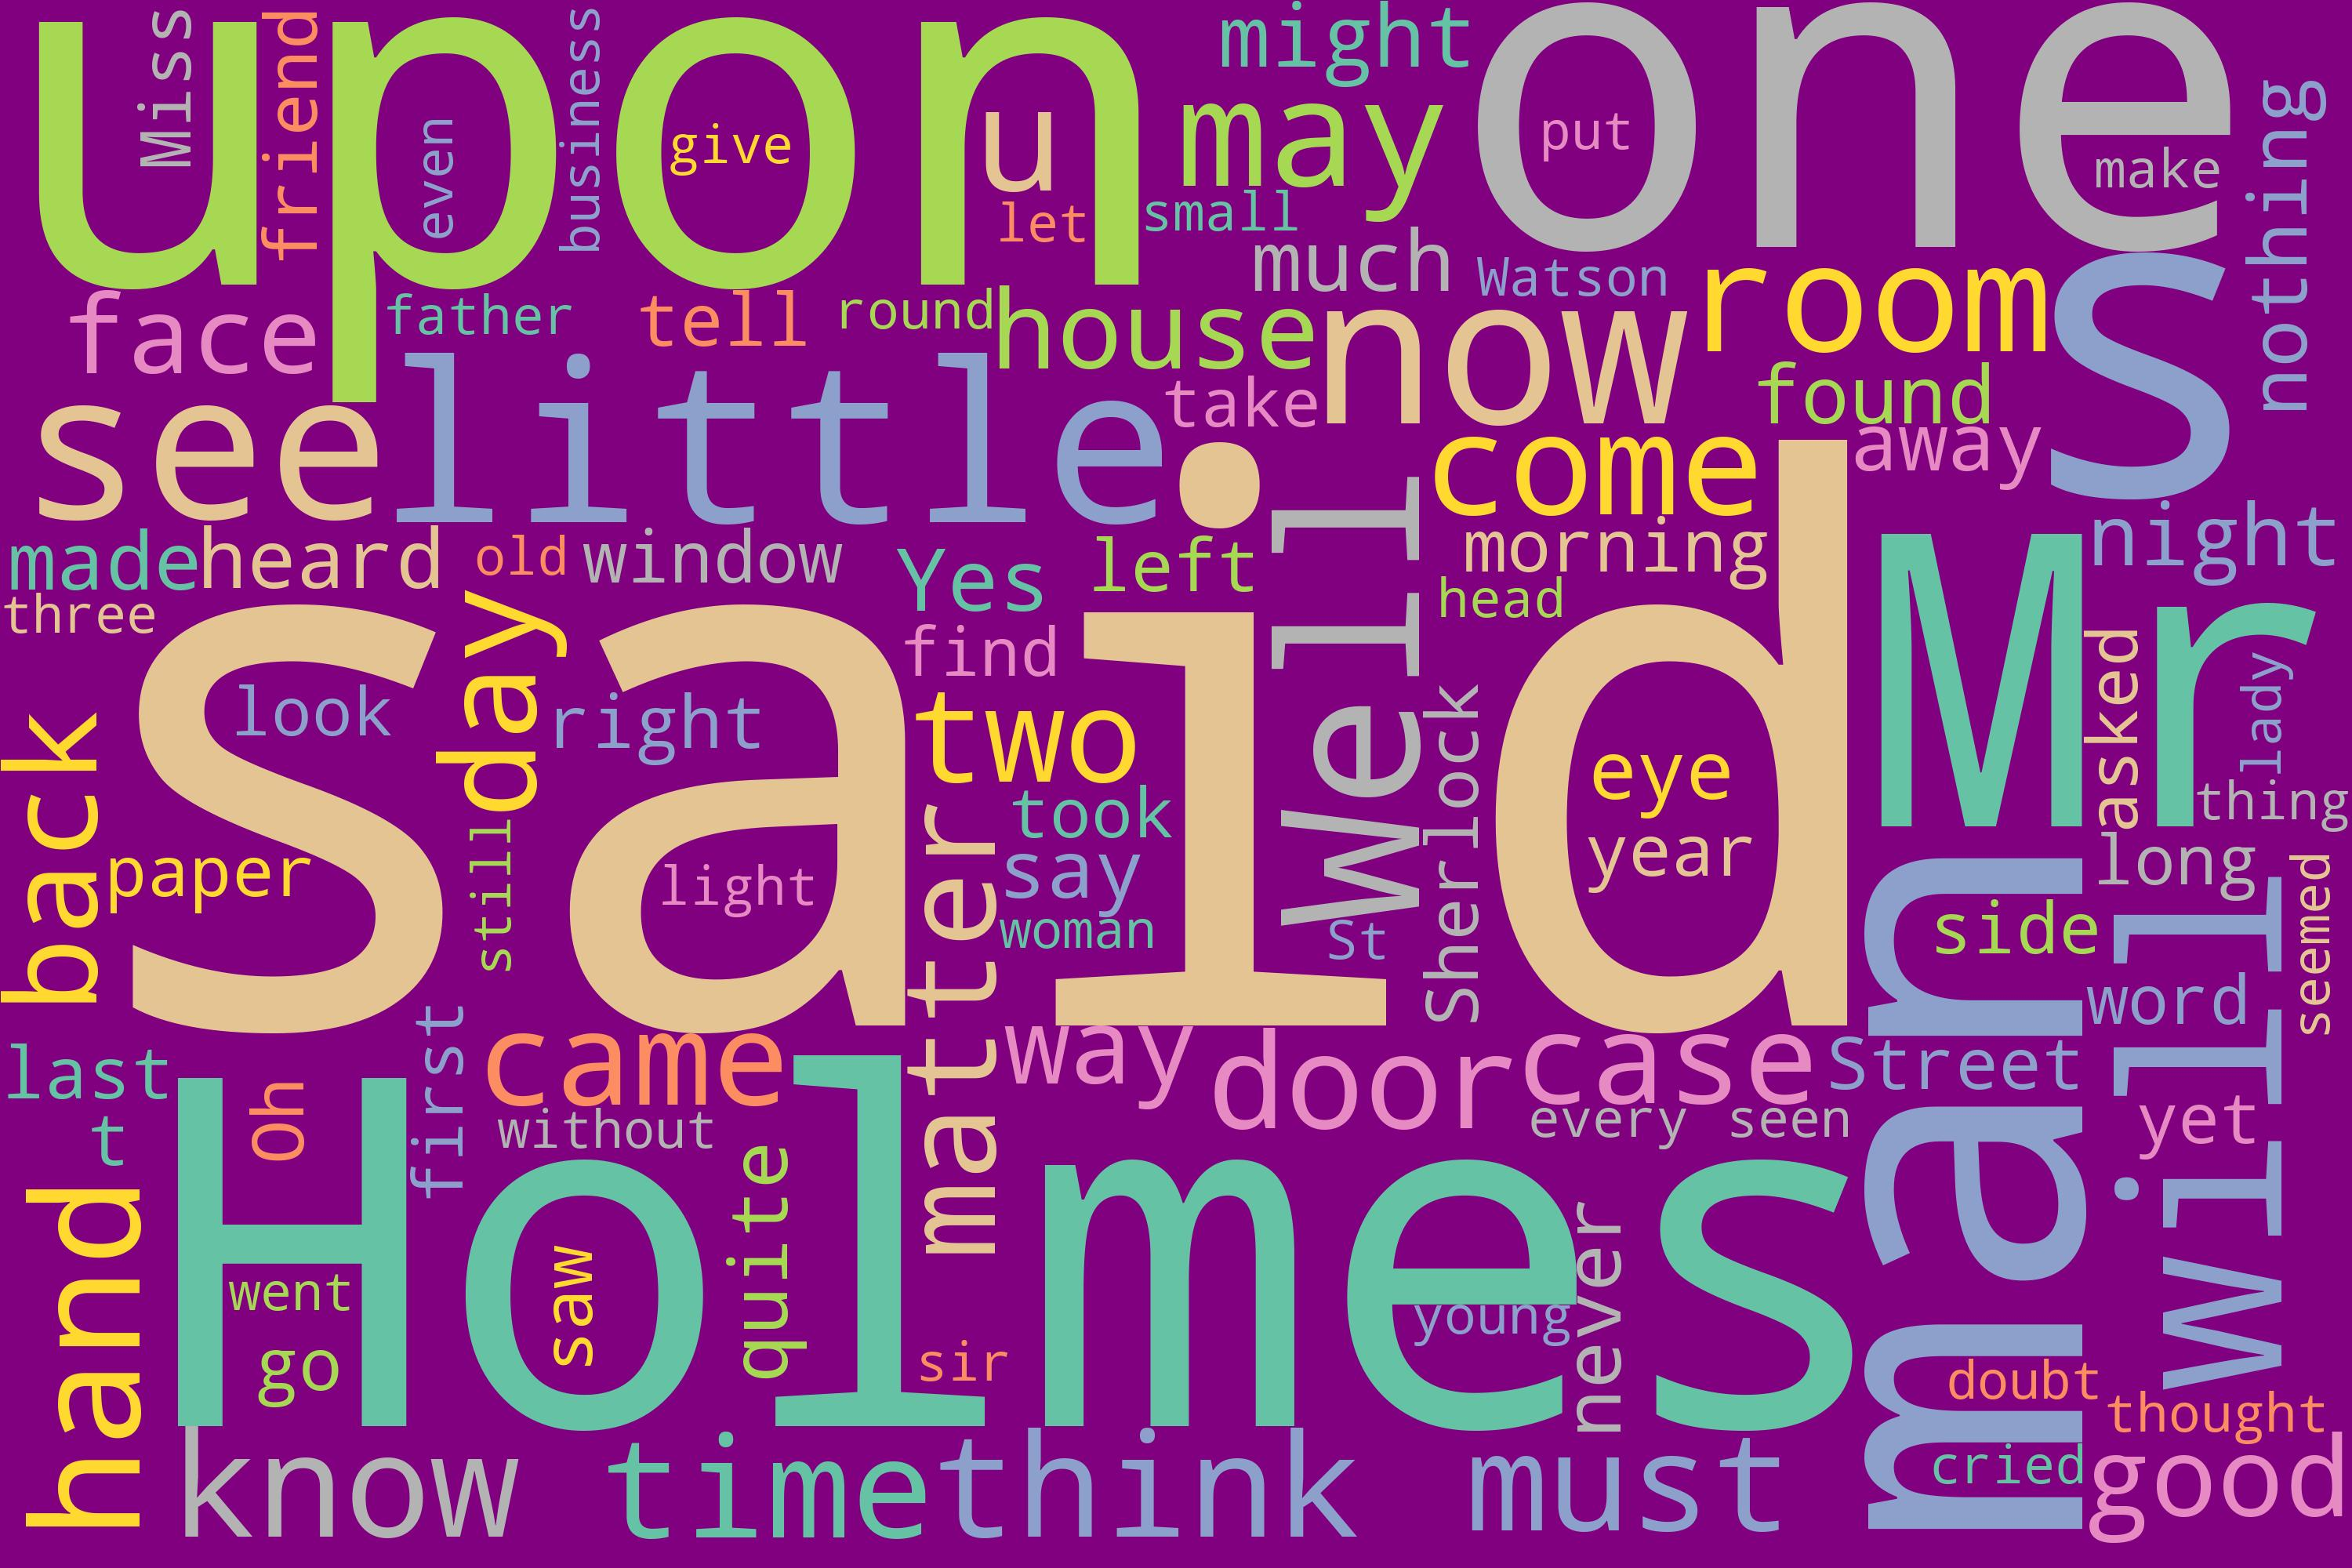
\includegraphics[width = 0.7\textwidth]{Images/SherlockHolmes_ArthurDoyle.jpeg} % enter the filename here
		\caption{Word Cloud - Sherlock Holmes}
		\label{fig:sherlock-holmes}
	\end{center}
\end{figure}

\begin{figure}[H]
	\begin{center}
		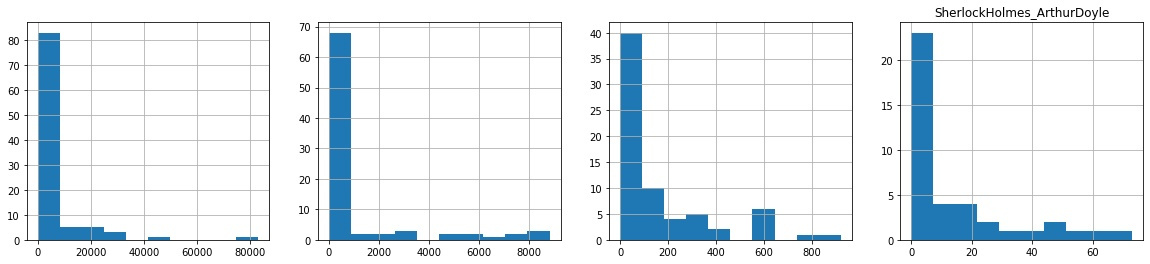
\includegraphics[width = 1.0\textwidth]{Images/char_hist_SherlockHolmes_ArthurDoyle.jpeg} % enter the filename here
		\caption{Character Histogram - Sherlock Holmes}
		\label{fig:histogram-sherlockholmes}
	\end{center}
\end{figure}

\subsection{\textcite{sign-of-the-four}} %enter the name of the subsection here
\label{sec:sign-of-the-four} % enter the subsection label here (for cross referencing)

The Sign of the Four is the second of Arthur Conan Doyle's Sherlock Holmes novels. In it, the detective and his companion Dr. Watson unravel a mystery of hidden treasure and murder. Miss Mary Morstan arrives at 221B, Baker Street to request help with the mystery of her missing father, her anonymous gifts of pearls, and a letter requesting her to meet an unknown person that evening. Holmes takes on her case and the adventure begins. Watson narrates the tale that sees the detective tracking down hidden treasure and murderers. By the end of the story the criminals are either dead or arrested, and Miss Mary Morstan and Watson are engaged to be married. \textcite{sign-of-the-four-summary}. Below is a quick word cloud from the complete book. 

\begin{figure}[H]
	\begin{center}
		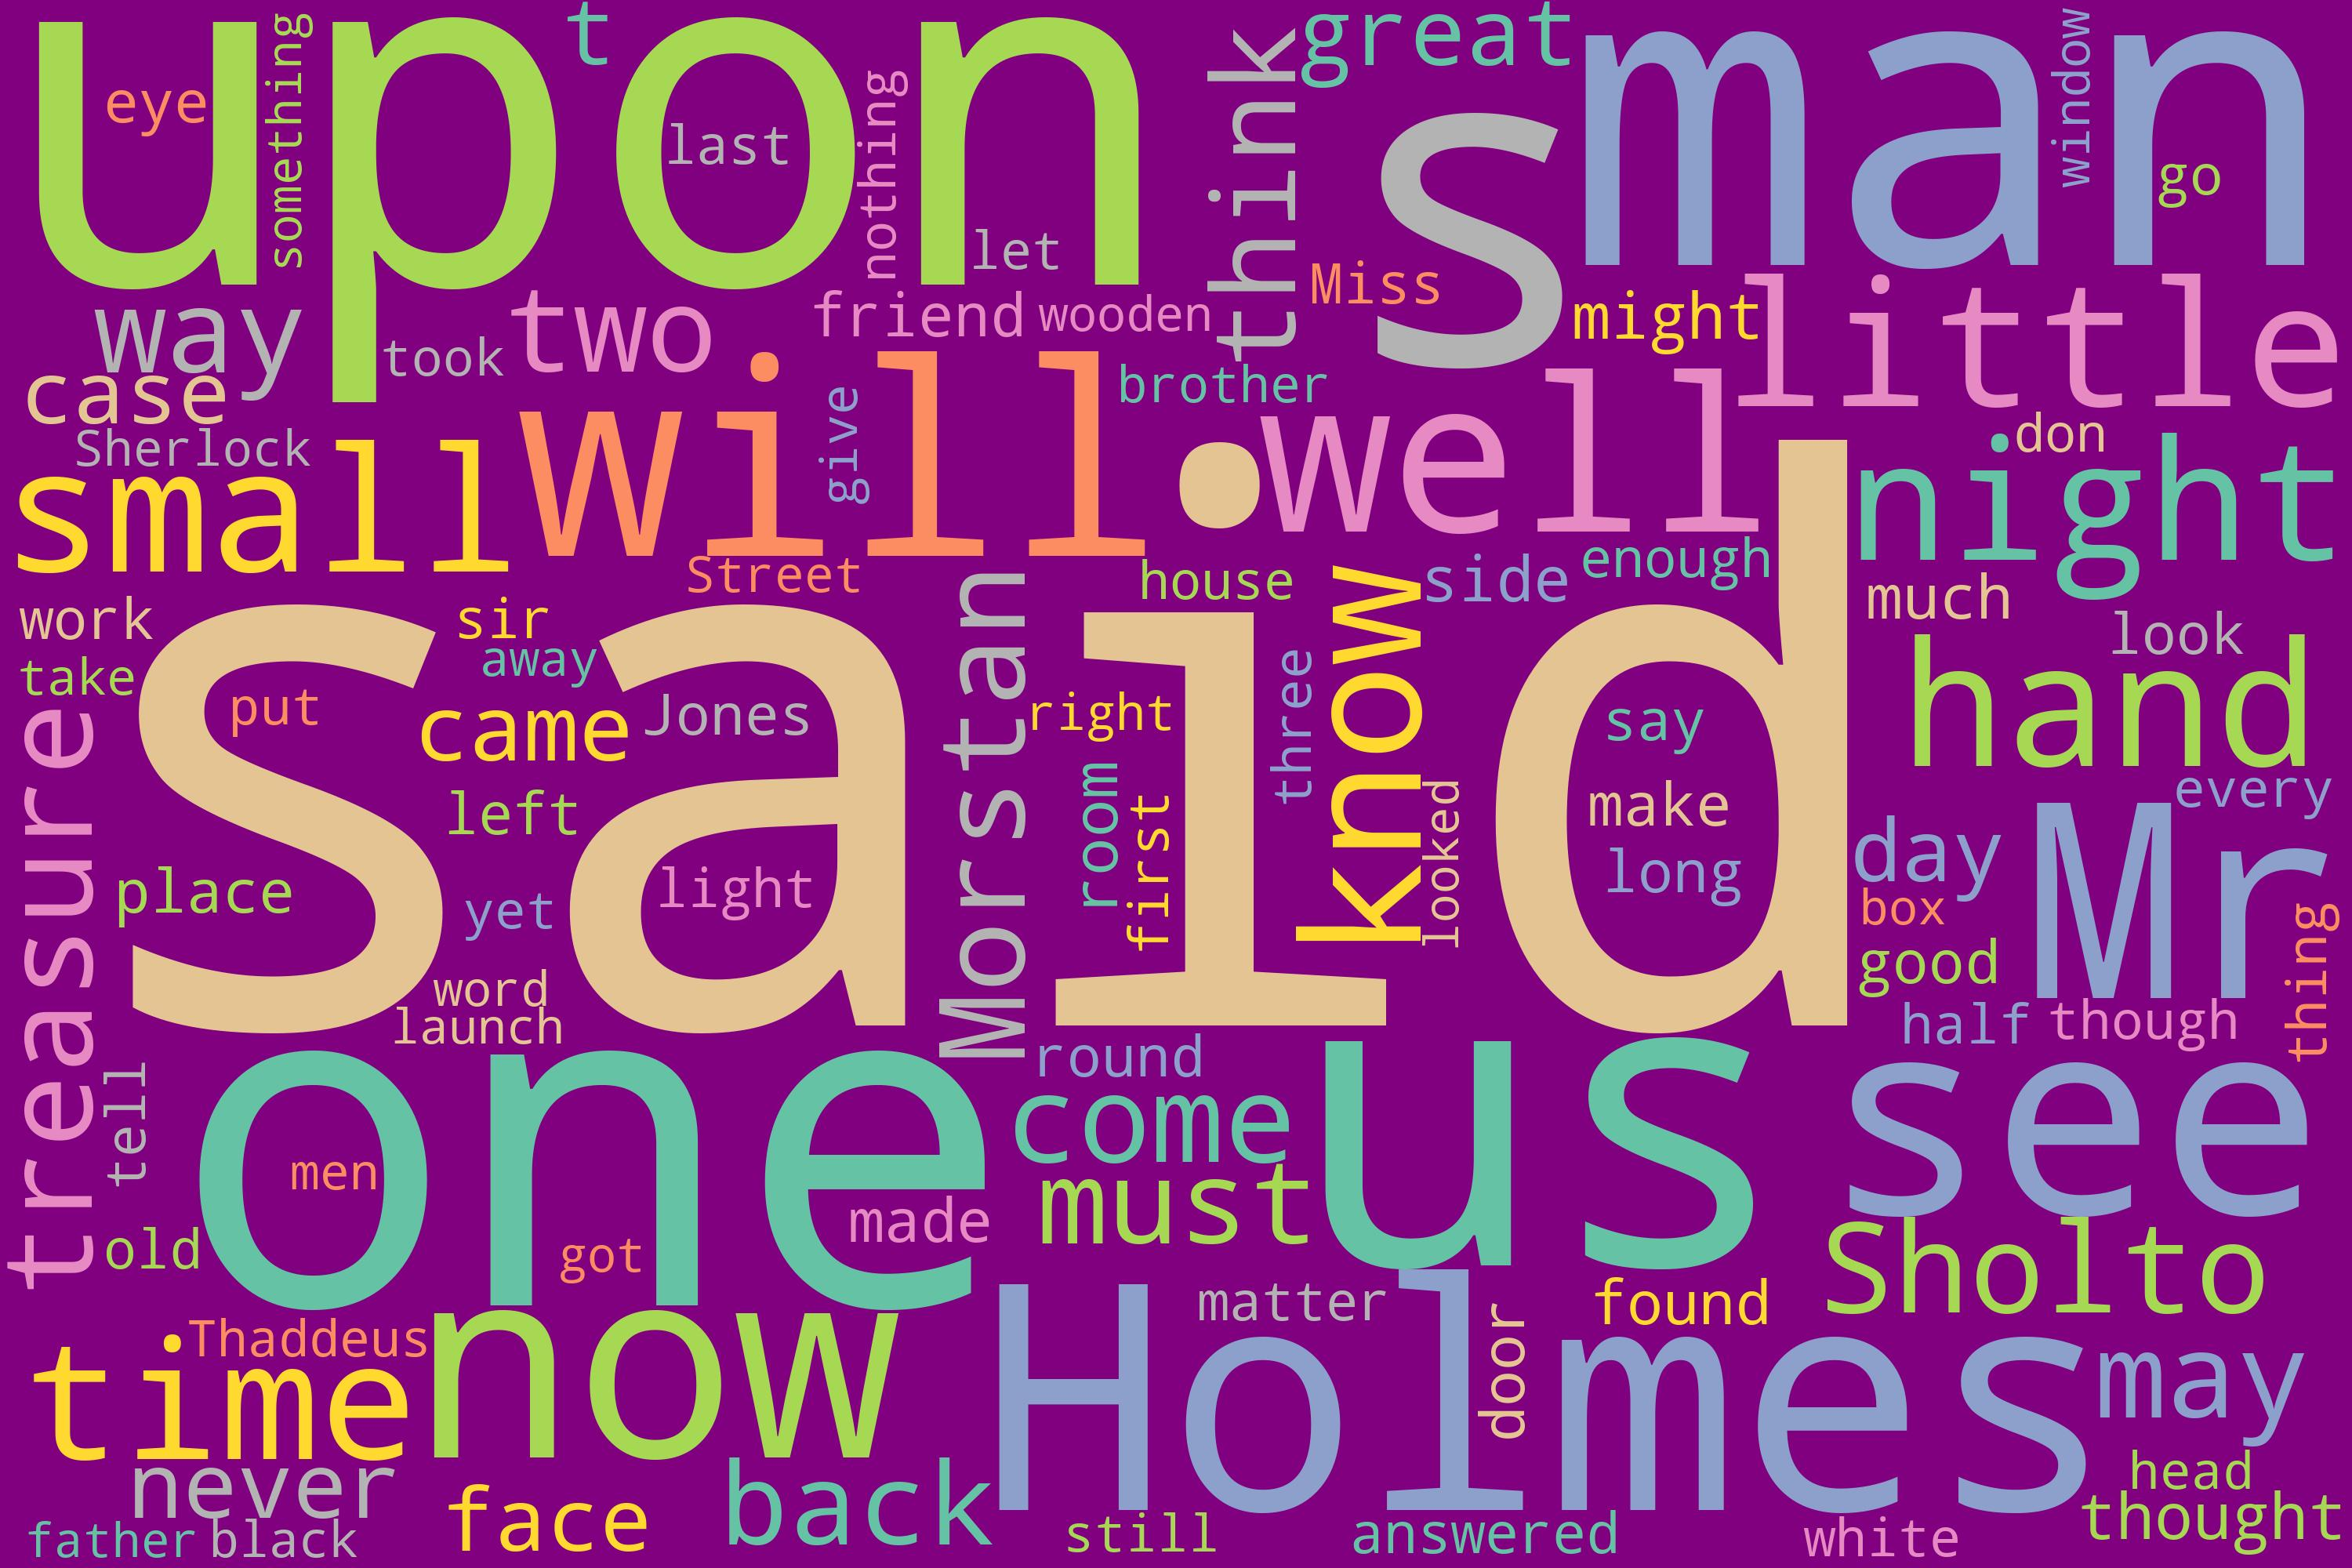
\includegraphics[width = 0.7\textwidth]{Images/SignOfTheFour_ArthurDoyle.jpeg} % enter the filename here
		\caption{Word Cloud - Sign of the Four}
		\label{fig:sign-of-the-four}
	\end{center}
\end{figure}

\begin{figure}[H]
	\begin{center}
		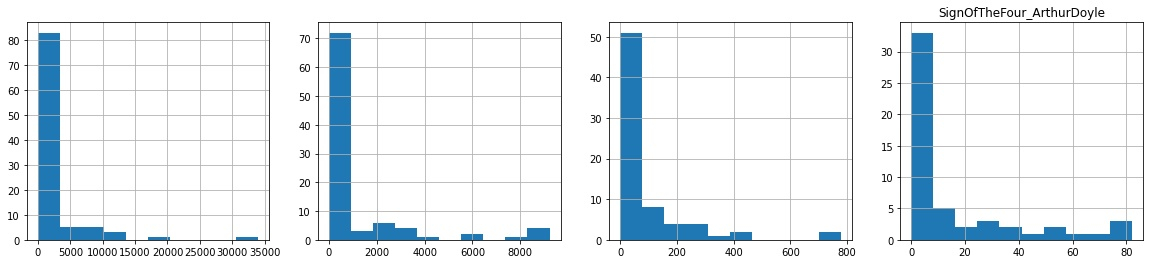
\includegraphics[width = 1.0\textwidth]{Images/char_hist_SignOfTheFour_ArthurDoyle.jpeg} % enter the filename here
		\caption{Character Histogram - Sign of the Four}
		\label{fig:histogram-signofthefour}
	\end{center}
\end{figure}

One key thing to notice is all of the histograms seem very skewed to the left. That's because a majority of the 98 characters do not actively occur in the entire text, mentioned in the section \ref{sec:unique-character-sets}. At maximum, we would see a corpus of 40 characters which would occur the most across all the text.
